\documentclass[a4paper,11pt]{article}
\usepackage[T1]{fontenc}
\usepackage[utf8]{inputenc}
\usepackage{lmodern}
\usepackage{textcomp}
\usepackage{amssymb}
\usepackage[margin=1.5cm]{geometry}
\usepackage{lscape}

\title{HICF1 -  Final Report v1}
\author{Dr. Susanne Weller}
\date{\today}

\usepackage{Sweave}
\begin{document}
\Sconcordance{concordance:HICF1_Finalreportv1.tex:HICF1_Finalreportv1.Rnw:%
1 13 1 1 0 1 1 1 2 2 1 1 39 1 28 1 4 63 0 1 2 1 1 1 43 1 4 64 0 1 2 2 1 %
1 4 64 0 1 2 14 1 1 18 1 12 1 3 2 1 1 4 1 38 1 18 1 4 64 0 1 2 1 12 1 2 %
3 1 1 33 6 1 1 52 1 5 54 0 1 2 4 1 1 14 1 5 14 0 1 2 140 1}

\maketitle

\section*{Univariate Analysis}


% Table created by stargazer v.5.1 by Marek Hlavac, Harvard University. E-mail: hlavac at fas.harvard.edu
% Date and time: Tue, Jul 29, 2014 - 16:08:11
\begin{table}[!htbp] \centering 
  \caption{Univariate Analysis against MRD outcome} 
  \label{} 
\tiny 
\begin{tabular}{@{\extracolsep{1p}} cccccccccc} 
\\[-1.8ex]\hline 
\hline \\[-1.8ex] 
 & p.value & uncorrected & corrected.p.value & corrected & MRDneg0 & MRDpos1 & MRDneg1 & sum & testused \\ 
\hline \\[-1.8ex] 
TP53\_ALL & $0.00004$ & \textasteriskcentered \textasteriskcentered \textasteriskcentered  & $0.002$ & \textasteriskcentered \textasteriskcentered  & $105$ & $19$ & $2$ & $209$ & Fisher's Exact Test \\ 
TP53\_del & $0.012$ & \textasteriskcentered  & $0.513$ & n.s. & $107$ & $6$ & $0$ & $209$ & Fisher's Exact Test \\ 
TP53\_cnLOH & $0.055$ & trend & $1$ & n.s. & $107$ & $4$ & $0$ & $209$ & Fisher's Exact Test \\ 
TP53\_mut & $0.00001$ & \textasteriskcentered \textasteriskcentered \textasteriskcentered  & $0.001$ & \textasteriskcentered \textasteriskcentered \textasteriskcentered  & $107$ & $15$ & $0$ & $209$ & Fisher's Exact Test \\ 
TP53\_bi & $0.009$ & \textasteriskcentered \textasteriskcentered  & $0.360$ & n.s. & $106$ & $9$ & $1$ & $209$ & Fisher's Exact Test \\ 
ATM\_ALL & $0.002$ & \textasteriskcentered \textasteriskcentered  & $0.085$ & trend & $83$ & $44$ & $24$ & $209$ & Fisher's Exact Test \\ 
ATM\_mut & $0.036$ & \textasteriskcentered  & $1$ & n.s. & $88$ & $31$ & $19$ & $209$ & Fisher's Exact Test \\ 
ATM\_del & $0.0005$ & \textasteriskcentered \textasteriskcentered \textasteriskcentered  & $0.022$ & \textasteriskcentered  & $98$ & $28$ & $9$ & $209$ & Fisher's Exact Test \\ 
ATM\_cnLOH & $0.203$ & n.s. & $1$ & n.s. & $106$ & $4$ & $1$ & $209$ & Fisher's Exact Test \\ 
ATM\_mt1 & $1$ & n.s. & $1$ & n.s. & $101$ & $5$ & $6$ & $209$ & Fisher's Exact Test \\ 
BIRC3\_ALL & $0.094$ & trend & $1$ & n.s. & $94$ & $22$ & $13$ & $209$ & Fisher's Exact Test \\ 
BIRC3\_mut & $0.375$ & n.s. & $1$ & n.s. & $99$ & $4$ & $8$ & $209$ & Fisher's Exact Test \\ 
BIRC3\_del & $0.002$ & \textasteriskcentered \textasteriskcentered  & $0.076$ & trend & $101$ & $21$ & $6$ & $209$ & Fisher's Exact Test \\ 
ATM\_bi & $0.002$ & \textasteriskcentered \textasteriskcentered  & $0.088$ & trend & $102$ & $19$ & $5$ & $209$ & Fisher's Exact Test \\ 
BIRC3\_bi & $0.360$ & n.s. & $1$ & n.s. & $106$ & $3$ & $1$ & $209$ & Fisher's Exact Test \\ 
X11q\_mono & $0.046$ & \textasteriskcentered  & $1$ & n.s. & $104$ & $10$ & $3$ & $209$ & Fisher's Exact Test \\ 
ATM\_mono & $0.836$ & n.s. & $1$ & n.s. & $93$ & $12$ & $14$ & $209$ & Fisher's Exact Test \\ 
BIRC3\_mono & $0.066$ & trend & $1$ & n.s. & $100$ & $1$ & $7$ & $209$ & Fisher's Exact Test \\ 
NOTCH1\_mut & $0.069$ & trend & $1$ & n.s. & $88$ & $9$ & $19$ & $209$ & Fisher's Exact Test \\ 
SF3B1\_mut & $0.415$ & n.s. & $1$ & n.s. & $85$ & $26$ & $22$ & $209$ & Fisher's Exact Test \\ 
X6q.\_del\_ALL & $0.595$ & n.s. & $1$ & n.s. & $98$ & $6$ & $9$ & $209$ & Fisher's Exact Test \\ 
X13q\_ALL & $0.267$ & n.s. & $1$ & n.s. & $54$ & $59$ & $53$ & $209$ & Fisher's Exact Test \\ 
X13del\_homo & $0.832$ & n.s. & $1$ & n.s. & $95$ & $13$ & $12$ & $209$ & Fisher's Exact Test \\ 
X13q\_het & $0.330$ & n.s. & $1$ & n.s. & $66$ & $46$ & $41$ & $209$ & Fisher's Exact Test \\ 
X13qdelRB1 & $0.743$ & n.s. & $1$ & n.s. & $84$ & $24$ & $23$ & $209$ & Fisher's Exact Test \\ 
X13q\_Ox & $0.248$ & n.s. & $1$ & n.s. & $88$ & $12$ & $19$ & $209$ & Fisher's Exact Test \\ 
X13q\_Rossi & $1$ & n.s. & $1$ & n.s. & $73$ & $32$ & $34$ & $209$ & Fisher's Exact Test \\ 
Trisomy\_12 & $0.002$ & \textasteriskcentered \textasteriskcentered  & $0.100$ & trend & $82$ & $8$ & $25$ & $209$ & Fisher's Exact Test \\ 
Trisomy\_18 & $0.060$ & trend & $1$ & n.s. & $102$ & $0$ & $5$ & $209$ & Fisher's Exact Test \\ 
Trisomy\_19 & $0.029$ & \textasteriskcentered  & $1$ & n.s. & $101$ & $0$ & $6$ & $209$ & Fisher's Exact Test \\ 
XPO1\_ALL & $0.160$ & n.s. & $1$ & n.s. & $100$ & $13$ & $7$ & $209$ & Fisher's Exact Test \\ 
XPO1\_gain & $0.054$ & trend & $1$ & n.s. & $105$ & $8$ & $2$ & $209$ & Fisher's Exact Test \\ 
XPO1\_mutation & $0.764$ & n.s. & $1$ & n.s. & $102$ & $6$ & $5$ & $209$ & Fisher's Exact Test \\ 
SAMHD1\_ALL & $0.054$ & trend & $1$ & n.s. & $105$ & $8$ & $2$ & $209$ & Fisher's Exact Test \\ 
SAMHD1\_mut & $0.006$ & \textasteriskcentered \textasteriskcentered  & $0.254$ & n.s. & $107$ & $7$ & $0$ & $209$ & Fisher's Exact Test \\ 
SAMHD1\_cnLOH\_Del & $0.437$ & n.s. & $1$ & n.s. & $105$ & $4$ & $2$ & $209$ & Fisher's Exact Test \\ 
MYD88\_mut & $1$ & n.s. & $1$ & n.s. & $105$ & $1$ & $2$ & $209$ & Fisher's Exact Test \\ 
MED12mutation & $0.360$ & n.s. & $1$ & n.s. & $106$ & $3$ & $1$ & $209$ & Fisher's Exact Test \\ 
X8q\_ALL & $0.323$ & n.s. & $1$ & n.s. & $104$ & $6$ & $3$ & $209$ & Fisher's Exact Test \\ 
X8q24\_gain & $0.203$ & n.s. & $1$ & n.s. & $106$ & $4$ & $1$ & $209$ & Fisher's Exact Test \\ 
ZFPM2\_mut & $1$ & n.s. & $1$ & n.s. & $105$ & $2$ & $2$ & $209$ & Fisher's Exact Test \\ 
Subclones & $0.050$ & trend & $1$ & n.s. & $$ & $$ & $$ & $$ & Wilcoxon Test \\ 
Total\_num\_CNAs & $0.483$ & n.s. & $1$ & n.s. & $$ & $$ & $$ & $$ & Wilcoxon Test \\ 
No\_alteration & $0.622$ & n.s. & $1$ & n.s. & $104$ & $1$ & $3$ & $209$ & Fisher's Exact Test \\ 
Binet & $0.770$ & n.s. & $1$ & n.s. & $72$ & $36$ & $35$ & $209$ & Fisher's Exact Test \\ 
age\_at\_randomisation & $0.100$ & trend & $1$ & n.s. & $$ & $$ & $$ & $$ & Wilcoxon Test \\ 
patient\_gender & $0.443$ & n.s. & $1$ & n.s. & $33$ & $76$ & $74$ & $209$ & Fisher's Exact Test \\ 
vh\_mutation\_status & $0.0003$ & \textasteriskcentered \textasteriskcentered \textasteriskcentered  & $0.015$ & \textasteriskcentered  & $55$ & $60$ & $40$ & $181$ & Fisher's Exact Test \\ 
ALC & $0.017$ & \textasteriskcentered  & $0.671$ & n.s. & $$ & $$ & $$ & $$ & Wilcoxon Test \\ 
WBC & $0.013$ & \textasteriskcentered  & $0.513$ & n.s. & $$ & $$ & $$ & $$ & Wilcoxon Test \\ 
cd38 & $0.707$ & n.s. & $1$ & n.s. & $45$ & $40$ & $59$ & $147$ & Fisher's Exact Test \\ 
\hline \\[-1.8ex] 
\end{tabular} 
\end{table} 
\section*{Associations}
\begin{landscape}
% Table created by stargazer v.5.1 by Marek Hlavac, Harvard University. E-mail: hlavac at fas.harvard.edu
% Date and time: Tue, Jul 29, 2014 - 16:08:13
\begin{table}[!htbp] \centering 
  \caption{Uncorrected p-values for association between genetic lesions} 
  \label{} 
\tiny 
\begin{tabular}{@{\extracolsep{1p}} cccccccccccccccccccccccccccccccccccccccccccccccccccccc} 
\\[-1.8ex]\hline 
\hline \\[-1.8ex] 
 & variables & TP53\_ALL & TP53\_del & TP53\_cnLOH & TP53\_mut & TP53\_bi & ATM\_ALL & ATM\_mut & ATM\_del & ATM\_cnLOH & ATM\_mt1 & BIRC3\_ALL & BIRC3\_mut & BIRC3\_del & ATM\_bi & BIRC3\_bi & X11q\_mono & ATM\_mono & BIRC3\_mono & NOTCH1\_mut & SF3B1\_mut & X6q.\_del\_ALL & X13q\_ALL & X13del\_homo & X13q\_het & X13qdelRB1 & X13q\_Ox & X13q\_Rossi & Trisomy\_12 & Trisomy\_18 & Trisomy\_19 & XPO1\_ALL & XPO1\_gain & XPO1\_mutation & SAMHD1\_ALL & SAMHD1\_mut & SAMHD1\_cnLOH\_Del & MYD88\_mut & MED12mutation & X8q\_ALL & X8q24\_gain & ZFPM2\_mut & Subclones & Total\_num\_CNAs & No\_alteration & Binet & age\_at\_randomisation & patient\_gender & vh\_mutation\_status & MRD & ALC & WBC & cd38 \\ 
\hline \\[-1.8ex] 
1 & TP53\_ALL & $$ & $0$ & $0.001$ & $0$ & $0$ & $0.510$ & $0.571$ & $0.498$ & $1$ & $0.411$ & $0.343$ & $1$ & $0.593$ & $0.386$ & $0.444$ & $1$ & $0.627$ & $0.636$ & $0.432$ & $0.422$ & $0.101$ & $0.690$ & $0.083$ & $0.655$ & $0.073$ & $0.038$ & $0$ & $0.143$ & $1$ & $1$ & $0.202$ & $0.031$ & $0.682$ & $1$ & $1$ & $1$ & $1$ & $0.198$ & $0.031$ & $0.006$ & $1$ & $0.009$ & $0$ & $1$ & $1$ & $0.773$ & $0.817$ & $0.234$ & $0.161$ & $0.861$ & $0.852$ & $0.292$ \\ 
2 & TP53\_del & $$ & $$ & $1$ & $0$ & $0$ & $0.274$ & $0.530$ & $0.429$ & $1$ & $1$ & $0.422$ & $1$ & $0.642$ & $0.634$ & $1$ & $1$ & $0.670$ & $1$ & $0.648$ & $0.181$ & $0.467$ & $0.825$ & $0.634$ & $1$ & $0.183$ & $0.412$ & $0.081$ & $0.417$ & $1$ & $1$ & $0.073$ & $0.009$ & $1$ & $0.444$ & $1$ & $0.342$ & $1$ & $1$ & $0.066$ & $0.027$ & $1$ & $0.021$ & $0$ & $1$ & $0.402$ & $0.705$ & $0.706$ & $0.275$ & $0.495$ & $0.494$ & $0.418$ & $1$ \\ 
3 & TP53\_cnLOH & $$ & $$ & $$ & $0.005$ & $0.002$ & $1$ & $0.632$ & $0.505$ & $1$ & $1$ & $1$ & $1$ & $1$ & $1$ & $1$ & $0.209$ & $1$ & $1$ & $0.101$ & $0.596$ & $1$ & $0.169$ & $1$ & $0.091$ & $0.609$ & $1$ & $0.638$ & $1$ & $1$ & $1$ & $1$ & $1$ & $1$ & $1$ & $1$ & $1$ & $1$ & $1$ & $0.154$ & $0.096$ & $1$ & $0.688$ & $0.189$ & $1$ & $1$ & $0.481$ & $0.769$ & $1$ & $0.134$ & $0.421$ & $0.323$ & $1$ \\ 
4 & TP53\_mut & $$ & $$ & $$ & $$ & $0$ & $0.173$ & $0.186$ & $0.275$ & $1$ & $0.631$ & $0.087$ & $0.642$ & $0.189$ & $0.181$ & $1$ & $1$ & $1$ & $1$ & $1$ & $1$ & $0.357$ & $0.875$ & $0.181$ & $0.377$ & $0.099$ & $0.125$ & $0.006$ & $0.083$ & $1$ & $1$ & $0.045$ & $0.010$ & $0.327$ & $1$ & $1$ & $0.568$ & $1$ & $1$ & $0.010$ & $0.002$ & $1$ & $0.002$ & $0$ & $1$ & $0.847$ & $0.661$ & $0.684$ & $0.215$ & $0.099$ & $0.484$ & $0.501$ & $0.878$ \\ 
5 & TP53\_bi & $$ & $$ & $$ & $$ & $$ & $0.642$ & $0.595$ & $0.527$ & $1$ & $0.505$ & $0.183$ & $1$ & $0.429$ & $0.416$ & $1$ & $0.560$ & $0.482$ & $1$ & $1$ & $0.386$ & $0.585$ & $1$ & $0.416$ & $0.536$ & $0.392$ & $0.276$ & $0.025$ & $0.181$ & $1$ & $1$ & $0.153$ & $0.022$ & $1$ & $0.560$ & $1$ & $0.444$ & $1$ & $1$ & $0.022$ & $0.006$ & $1$ & $0.028$ & $0$ & $1$ & $0.489$ & $0.978$ & $0.748$ & $0.581$ & $0.432$ & $0.576$ & $0.570$ & $1$ \\ 
6 & ATM\_ALL & $$ & $$ & $$ & $$ & $$ & $$ & $0$ & $0$ & $0.031$ & $0.001$ & $0$ & $0.373$ & $0$ & $0$ & $0.031$ & $0$ & $0$ & $0.593$ & $0.441$ & $0.548$ & $0.655$ & $0.803$ & $0.740$ & $0.855$ & $0.192$ & $0$ & $0.832$ & $0.045$ & $0.281$ & $0.186$ & $0.858$ & $1$ & $1$ & $0.350$ & $0.209$ & $0.168$ & $1$ & $0.314$ & $0.782$ & $1$ & $0.405$ & $0.221$ & $0.080$ & $0.653$ & $0.230$ & $0.415$ & $0.264$ & $0.566$ & $0.546$ & $0.306$ & $0.115$ & $0.367$ \\ 
7 & ATM\_mut & $$ & $$ & $$ & $$ & $$ & $$ & $$ & $0.003$ & $0.011$ & $0$ & $0.111$ & $0.197$ & $0.017$ & $0$ & $0.647$ & $0.058$ & $0$ & $0.530$ & $0.157$ & $0.584$ & $0.605$ & $0.516$ & $0.251$ & $0.918$ & $0.348$ & $0$ & $0.094$ & $0.051$ & $0.416$ & $0.272$ & $0.677$ & $0.750$ & $0.790$ & $0.426$ & $0.473$ & $0.342$ & $1$ & $0.115$ & $1$ & $0.674$ & $0.632$ & $0.333$ & $0.305$ & $0.632$ & $0.652$ & $0.665$ & $0.511$ & $0.783$ & $0.923$ & $0.146$ & $0.069$ & $0.410$ \\ 
8 & ATM\_del & $$ & $$ & $$ & $$ & $$ & $$ & $$ & $$ & $1$ & $0.283$ & $0$ & $0.018$ & $0$ & $0$ & $0.002$ & $0$ & $0.002$ & $0.697$ & $0.829$ & $0.404$ & $0.342$ & $1$ & $0.345$ & $0.538$ & $0.189$ & $0.005$ & $0.384$ & $0.074$ & $0.632$ & $0.640$ & $0.200$ & $1$ & $0.187$ & $0.103$ & $0.167$ & $0.101$ & $1$ & $1$ & $0.697$ & $0.632$ & $0.157$ & $0.003$ & $0$ & $1$ & $0.172$ & $0.433$ & $0.383$ & $0.190$ & $0.084$ & $0.941$ & $0.663$ & $0.191$ \\ 
9 & ATM\_cnLOH & $$ & $$ & $$ & $$ & $$ & $$ & $$ & $$ & $$ & $1$ & $1$ & $1$ & $1$ & $0$ & $1$ & $1$ & $1$ & $1$ & $1$ & $0.312$ & $1$ & $0.348$ & $0.432$ & $0.474$ & $1$ & $1$ & $0.192$ & $1$ & $1$ & $1$ & $1$ & $1$ & $1$ & $1$ & $1$ & $1$ & $1$ & $1$ & $0.189$ & $0.118$ & $1$ & $0.684$ & $0.224$ & $1$ & $1$ & $0.594$ & $0.788$ & $1$ & $0.315$ & $0.777$ & $0.717$ & $0.207$ \\ 
10 & ATM\_mt1 & $$ & $$ & $$ & $$ & $$ & $$ & $$ & $$ & $$ & $$ & $0.277$ & $1$ & $0.413$ & $0.650$ & $1$ & $1$ & $0$ & $1$ & $1$ & $0.353$ & $1$ & $0.544$ & $0.393$ & $0.649$ & $0.065$ & $0.425$ & $0.183$ & $0.273$ & $1$ & $1$ & $1$ & $1$ & $0.505$ & $0.505$ & $0.331$ & $0.395$ & $1$ & $0.049$ & $1$ & $1$ & $1$ & $0.066$ & $0.217$ & $1$ & $1$ & $0.646$ & $0.863$ & $0.693$ & $1$ & $0.323$ & $0.333$ & $0.693$ \\ 
11 & BIRC3\_ALL & $$ & $$ & $$ & $$ & $$ & $$ & $$ & $$ & $$ & $$ & $$ & $0$ & $0$ & $0$ & $0.002$ & $0$ & $0.003$ & $0$ & $0.662$ & $1$ & $0.743$ & $0.821$ & $0.338$ & $0.706$ & $0.507$ & $0.005$ & $0.180$ & $0.688$ & $0.266$ & $0.114$ & $0.195$ & $1$ & $0.183$ & $0.088$ & $0.152$ & $0.089$ & $1$ & $0.636$ & $0.236$ & $0.631$ & $0.030$ & $0.075$ & $0.019$ & $1$ & $0.577$ & $0.653$ & $0.553$ & $0.501$ & $0.554$ & $0.744$ & $0.889$ & $0.738$ \\ 
12 & BIRC3\_mut & $$ & $$ & $$ & $$ & $$ & $$ & $$ & $$ & $$ & $$ & $$ & $$ & $0.042$ & $1$ & $0$ & $1$ & $0.182$ & $0$ & $0.053$ & $1$ & $0.611$ & $0.858$ & $1$ & $1$ & $1$ & $0.284$ & $0.027$ & $0.034$ & $0.055$ & $0.010$ & $0.412$ & $1$ & $1$ & $0.585$ & $1$ & $0.467$ & $1$ & $1$ & $0.131$ & $1$ & $0.027$ & $0.969$ & $0.073$ & $1$ & $1$ & $0.871$ & $0.755$ & $0.593$ & $0.261$ & $0.251$ & $0.360$ & $0.291$ \\ 
13 & BIRC3\_del & $$ & $$ & $$ & $$ & $$ & $$ & $$ & $$ & $$ & $$ & $$ & $$ & $$ & $0$ & $0$ & $0$ & $0.017$ & $0.642$ & $0.449$ & $0.845$ & $0.713$ & $0.897$ & $0.273$ & $0.664$ & $0.439$ & $0.025$ & $0.611$ & $0.100$ & $1$ & $1$ & $0.380$ & $1$ & $0.429$ & $0.101$ & $0.081$ & $0.132$ & $1$ & $1$ & $1$ & $1$ & $0.395$ & $0.018$ & $0.075$ & $1$ & $0.422$ & $0.548$ & $0.368$ & $0.160$ & $0.103$ & $0.836$ & $0.566$ & $0.444$ \\ 
14 & ATM\_bi & $$ & $$ & $$ & $$ & $$ & $$ & $$ & $$ & $$ & $$ & $$ & $$ & $$ & $$ & $1$ & $0.416$ & $0.025$ & $1$ & $0.594$ & $0.216$ & $0.241$ & $0.496$ & $1$ & $0.445$ & $0.422$ & $0.037$ & $0.154$ & $0.025$ & $1$ & $1$ & $0.529$ & $1$ & $0.416$ & $0.212$ & $0.596$ & $0.312$ & $1$ & $0.547$ & $1$ & $0.493$ & $1$ & $0.004$ & $0$ & $1$ & $0.613$ & $0.574$ & $0.724$ & $0.419$ & $0.116$ & $0.483$ & $0.394$ & $0.505$ \\ 
15 & BIRC3\_bi & $$ & $$ & $$ & $$ & $$ & $$ & $$ & $$ & $$ & $$ & $$ & $$ & $$ & $$ & $$ & $1$ & $1$ & $1$ & $0.488$ & $1$ & $1$ & $1$ & $1$ & $1$ & $1$ & $1$ & $0.413$ & $1$ & $1$ & $1$ & $1$ & $1$ & $1$ & $1$ & $1$ & $1$ & $1$ & $1$ & $1$ & $1$ & $1$ & $0.454$ & $0.303$ & $1$ & $1$ & $0.624$ & $1$ & $0.758$ & $0.740$ & $0.532$ & $0.558$ & $0.361$ \\ 
16 & X11q\_mono & $$ & $$ & $$ & $$ & $$ & $$ & $$ & $$ & $$ & $$ & $$ & $$ & $$ & $$ & $$ & $$ & $0.287$ & $1$ & $0.712$ & $0.564$ & $0.585$ & $1$ & $0.416$ & $0.536$ & $0.150$ & $0.276$ & $0.025$ & $0.731$ & $1$ & $1$ & $0.649$ & $1$ & $1$ & $0.198$ & $0.081$ & $0.117$ & $1$ & $1$ & $0.444$ & $1$ & $0.209$ & $0.977$ & $0.398$ & $1$ & $0.251$ & $0.374$ & $0.202$ & $0.581$ & $0.238$ & $0.878$ & $0.616$ & $0.461$ \\ 
17 & ATM\_mono & $$ & $$ & $$ & $$ & $$ & $$ & $$ & $$ & $$ & $$ & $$ & $$ & $$ & $$ & $$ & $$ & $$ & $0.415$ & $0.252$ & $0.859$ & $1$ & $0.907$ & $0.206$ & $0.600$ & $0.602$ & $0.012$ & $0.356$ & $0.672$ & $1$ & $0.633$ & $0.177$ & $0.670$ & $0.174$ & $0.482$ & $0.351$ & $0.203$ & $0.462$ & $0.096$ & $1$ & $0.606$ & $1$ & $0.316$ & $0.107$ & $1$ & $1$ & $0.878$ & $0.539$ & $0.728$ & $0.176$ & $0.176$ & $0.096$ & $0.818$ \\ 
18 & BIRC3\_mono & $$ & $$ & $$ & $$ & $$ & $$ & $$ & $$ & $$ & $$ & $$ & $$ & $$ & $$ & $$ & $$ & $$ & $$ & $0.047$ & $1$ & $0.467$ & $1$ & $1$ & $1$ & $1$ & $0.412$ & $0.081$ & $0.006$ & $0.027$ & $0.003$ & $1$ & $1$ & $1$ & $0.444$ & $1$ & $0.342$ & $1$ & $1$ & $0.066$ & $1$ & $0.012$ & $0.558$ & $0.151$ & $1$ & $0.591$ & $0.879$ & $0.850$ & $0.387$ & $0.102$ & $0.347$ & $0.491$ & $0.512$ \\ 
19 & NOTCH1\_mut & $$ & $$ & $$ & $$ & $$ & $$ & $$ & $$ & $$ & $$ & $$ & $$ & $$ & $$ & $$ & $$ & $$ & $$ & $$ & $0.129$ & $0.728$ & $0.078$ & $0.279$ & $0.261$ & $0.458$ & $0.017$ & $0$ & $0.020$ & $0.553$ & $0.609$ & $1$ & $0.387$ & $1$ & $1$ & $1$ & $0.648$ & $1$ & $0.609$ & $1$ & $1$ & $0.415$ & $0.089$ & $0.917$ & $1$ & $0.029$ & $0.780$ & $0.828$ & $0.265$ & $0.088$ & $0.565$ & $0.493$ & $1$ \\ 
20 & SF3B1\_mut & $$ & $$ & $$ & $$ & $$ & $$ & $$ & $$ & $$ & $$ & $$ & $$ & $$ & $$ & $$ & $$ & $$ & $$ & $$ & $$ & $0.160$ & $0.843$ & $0.537$ & $0.443$ & $0.145$ & $0.001$ & $0$ & $0.003$ & $1$ & $1$ & $1$ & $0.181$ & $0.253$ & $0.386$ & $0.434$ & $0.732$ & $1$ & $0.674$ & $0.295$ & $0.393$ & $0.229$ & $0.845$ & $0.123$ & $1$ & $0.544$ & $0.059$ & $0.662$ & $0.142$ & $1$ & $0.192$ & $0.335$ & $0.379$ \\ 
21 & X6q.\_del\_ALL & $$ & $$ & $$ & $$ & $$ & $$ & $$ & $$ & $$ & $$ & $$ & $$ & $$ & $$ & $$ & $$ & $$ & $$ & $$ & $$ & $$ & $1$ & $1$ & $0.687$ & $1$ & $0.284$ & $1$ & $0.737$ & $1$ & $1$ & $1$ & $0.467$ & $1$ & $0.585$ & $1$ & $0.467$ & $1$ & $1$ & $0.467$ & $1$ & $0.222$ & $0.520$ & $0$ & $1$ & $0.823$ & $0.222$ & $0.755$ & $0.289$ & $0.850$ & $0.181$ & $0.194$ & $0.593$ \\ 
22 & X13q\_ALL & $$ & $$ & $$ & $$ & $$ & $$ & $$ & $$ & $$ & $$ & $$ & $$ & $$ & $$ & $$ & $$ & $$ & $$ & $$ & $$ & $$ & $$ & $0.002$ & $0$ & $0$ & $0.001$ & $0$ & $0$ & $1$ & $1$ & $0.382$ & $0.662$ & $0.349$ & $0.851$ & $0.624$ & $0.662$ & $0.169$ & $0.059$ & $0.662$ & $0.260$ & $0.730$ & $0$ & $0.001$ & $0.285$ & $0.867$ & $0.142$ & $0.842$ & $0.077$ & $0.659$ & $0.027$ & $0.047$ & $0.156$ \\ 
23 & X13del\_homo & $$ & $$ & $$ & $$ & $$ & $$ & $$ & $$ & $$ & $$ & $$ & $$ & $$ & $$ & $$ & $$ & $$ & $$ & $$ & $$ & $$ & $$ & $$ & $0$ & $0.152$ & $0.001$ & $0$ & $0.139$ & $1$ & $1$ & $0.336$ & $0.312$ & $0.674$ & $1$ & $1$ & $1$ & $0.364$ & $1$ & $0.634$ & $1$ & $1$ & $0.010$ & $0.378$ & $1$ & $0.502$ & $0.608$ & $0.814$ & $0.080$ & $1$ & $0.646$ & $0.610$ & $0.108$ \\ 
24 & X13q\_het & $$ & $$ & $$ & $$ & $$ & $$ & $$ & $$ & $$ & $$ & $$ & $$ & $$ & $$ & $$ & $$ & $$ & $$ & $$ & $$ & $$ & $$ & $$ & $$ & $0$ & $0.055$ & $0$ & $0.001$ & $0.744$ & $0.772$ & $0.622$ & $1$ & $0.398$ & $0.536$ & $0.399$ & $0.620$ & $0.240$ & $0.129$ & $0.325$ & $0.113$ & $1$ & $0.002$ & $0.004$ & $0.423$ & $1$ & $0.249$ & $0.624$ & $0.444$ & $0.632$ & $0.054$ & $0.094$ & $0.541$ \\ 
25 & X13qdelRB1 & $$ & $$ & $$ & $$ & $$ & $$ & $$ & $$ & $$ & $$ & $$ & $$ & $$ & $$ & $$ & $$ & $$ & $$ & $$ & $$ & $$ & $$ & $$ & $$ & $$ & $0.100$ & $0.005$ & $0.003$ & $0.655$ & $0.420$ & $0.664$ & $0.735$ & $0.270$ & $1$ & $0.442$ & $1$ & $0.241$ & $0.420$ & $1$ & $1$ & $0.609$ & $0.027$ & $0.040$ & $1$ & $0.476$ & $0.575$ & $0.302$ & $0.100$ & $0.611$ & $0.647$ & $0.617$ & $0.700$ \\ 
26 & X13q\_Ox & $$ & $$ & $$ & $$ & $$ & $$ & $$ & $$ & $$ & $$ & $$ & $$ & $$ & $$ & $$ & $$ & $$ & $$ & $$ & $$ & $$ & $$ & $$ & $$ & $$ & $$ & $0$ & $0.008$ & $1$ & $1$ & $0.085$ & $0.412$ & $0.276$ & $0.276$ & $0.635$ & $0.412$ & $1$ & $1$ & $0.412$ & $1$ & $1$ & $0.001$ & $0.509$ & $1$ & $0.452$ & $0.057$ & $0.832$ & $0.008$ & $0.307$ & $0.162$ & $0.279$ & $0.054$ \\ 
27 & X13q\_Rossi & $$ & $$ & $$ & $$ & $$ & $$ & $$ & $$ & $$ & $$ & $$ & $$ & $$ & $$ & $$ & $$ & $$ & $$ & $$ & $$ & $$ & $$ & $$ & $$ & $$ & $$ & $$ & $0$ & $1$ & $0.283$ & $0.848$ & $1$ & $1$ & $0.208$ & $0.311$ & $0.234$ & $0.034$ & $0.283$ & $0.381$ & $1$ & $0.638$ & $0$ & $0.220$ & $0.638$ & $0.340$ & $0.943$ & $0.938$ & $0.099$ & $0.648$ & $0.003$ & $0.017$ & $0.029$ \\ 
28 & Trisomy\_12 & $$ & $$ & $$ & $$ & $$ & $$ & $$ & $$ & $$ & $$ & $$ & $$ & $$ & $$ & $$ & $$ & $$ & $$ & $$ & $$ & $$ & $$ & $$ & $$ & $$ & $$ & $$ & $$ & $0.016$ & $0.001$ & $0.057$ & $0.417$ & $0.181$ & $0.181$ & $0.643$ & $0.417$ & $1$ & $0.102$ & $0.675$ & $0.616$ & $0.471$ & $0.002$ & $0.274$ & $1$ & $0.775$ & $0.633$ & $0.840$ & $0.303$ & $0.007$ & $0.028$ & $0.038$ & $0.424$ \\ 
29 & Trisomy\_18 & $$ & $$ & $$ & $$ & $$ & $$ & $$ & $$ & $$ & $$ & $$ & $$ & $$ & $$ & $$ & $$ & $$ & $$ & $$ & $$ & $$ & $$ & $$ & $$ & $$ & $$ & $$ & $$ & $$ & $0$ & $1$ & $1$ & $1$ & $1$ & $1$ & $1$ & $0.096$ & $1$ & $1$ & $1$ & $1$ & $0.462$ & $0.010$ & $1$ & $0.153$ & $0.924$ & $0.630$ & $0.086$ & $0.128$ & $0.015$ & $0.022$ & $0.272$ \\ 
30 & Trisomy\_19 & $$ & $$ & $$ & $$ & $$ & $$ & $$ & $$ & $$ & $$ & $$ & $$ & $$ & $$ & $$ & $$ & $$ & $$ & $$ & $$ & $$ & $$ & $$ & $$ & $$ & $$ & $$ & $$ & $$ & $$ & $1$ & $1$ & $1$ & $1$ & $1$ & $1$ & $1$ & $1$ & $1$ & $1$ & $1$ & $0.725$ & $0.052$ & $1$ & $0.521$ & $0.934$ & $1$ & $0.037$ & $0.055$ & $0.053$ & $0.069$ & $0.196$ \\ 
31 & XPO1\_ALL & $$ & $$ & $$ & $$ & $$ & $$ & $$ & $$ & $$ & $$ & $$ & $$ & $$ & $$ & $$ & $$ & $$ & $$ & $$ & $$ & $$ & $$ & $$ & $$ & $$ & $$ & $$ & $$ & $$ & $$ & $$ & $0$ & $0$ & $1$ & $0.538$ & $1$ & $1$ & $0.491$ & $0.619$ & $0.439$ & $1$ & $0.246$ & $0.451$ & $1$ & $0.589$ & $0.861$ & $0.899$ & $0.146$ & $0.540$ & $0.136$ & $0.104$ & $0.563$ \\ 
32 & XPO1\_gain & $$ & $$ & $$ & $$ & $$ & $$ & $$ & $$ & $$ & $$ & $$ & $$ & $$ & $$ & $$ & $$ & $$ & $$ & $$ & $$ & $$ & $$ & $$ & $$ & $$ & $$ & $$ & $$ & $$ & $$ & $$ & $$ & $0.444$ & $0.444$ & $0.285$ & $1$ & $1$ & $1$ & $0.342$ & $0.222$ & $1$ & $0.043$ & $0.001$ & $1$ & $1$ & $0.135$ & $0.706$ & $0.275$ & $0.162$ & $0.611$ & $0.593$ & $0.827$ \\ 
33 & XPO1\_mutation & $$ & $$ & $$ & $$ & $$ & $$ & $$ & $$ & $$ & $$ & $$ & $$ & $$ & $$ & $$ & $$ & $$ & $$ & $$ & $$ & $$ & $$ & $$ & $$ & $$ & $$ & $$ & $$ & $$ & $$ & $$ & $$ & $$ & $1$ & $1$ & $1$ & $1$ & $0.337$ & $1$ & $1$ & $1$ & $0.844$ & $0.144$ & $1$ & $0.489$ & $0.057$ & $1$ & $0.202$ & $1$ & $0.057$ & $0.044$ & $0.202$ \\ 
34 & SAMHD1\_ALL & $$ & $$ & $$ & $$ & $$ & $$ & $$ & $$ & $$ & $$ & $$ & $$ & $$ & $$ & $$ & $$ & $$ & $$ & $$ & $$ & $$ & $$ & $$ & $$ & $$ & $$ & $$ & $$ & $$ & $$ & $$ & $$ & $$ & $$ & $0$ & $0$ & $0.209$ & $0.337$ & $0.117$ & $1$ & $0.023$ & $0.816$ & $0.238$ & $1$ & $0.489$ & $0.164$ & $1$ & $0.854$ & $0.561$ & $0.026$ & $0.140$ & $0.138$ \\ 
35 & SAMHD1\_mut & $$ & $$ & $$ & $$ & $$ & $$ & $$ & $$ & $$ & $$ & $$ & $$ & $$ & $$ & $$ & $$ & $$ & $$ & $$ & $$ & $$ & $$ & $$ & $$ & $$ & $$ & $$ & $$ & $$ & $$ & $$ & $$ & $$ & $$ & $$ & $0$ & $1$ & $1$ & $0.285$ & $1$ & $0.125$ & $0.784$ & $0.422$ & $1$ & $1$ & $0.975$ & $0.529$ & $0.462$ & $0.119$ & $0.171$ & $0.123$ & $0.220$ \\ 
36 & SAMHD1\_cnLOH\_Del & $$ & $$ & $$ & $$ & $$ & $$ & $$ & $$ & $$ & $$ & $$ & $$ & $$ & $$ & $$ & $$ & $$ & $$ & $$ & $$ & $$ & $$ & $$ & $$ & $$ & $$ & $$ & $$ & $$ & $$ & $$ & $$ & $$ & $$ & $$ & $$ & $0.154$ & $0.254$ & $0.342$ & $1$ & $0.154$ & $0.609$ & $0.205$ & $1$ & $0.591$ & $0.459$ & $1$ & $1$ & $1$ & $0.137$ & $0.537$ & $0.276$ \\ 
37 & MYD88\_mut & $$ & $$ & $$ & $$ & $$ & $$ & $$ & $$ & $$ & $$ & $$ & $$ & $$ & $$ & $$ & $$ & $$ & $$ & $$ & $$ & $$ & $$ & $$ & $$ & $$ & $$ & $$ & $$ & $$ & $$ & $$ & $$ & $$ & $$ & $$ & $$ & $$ & $1$ & $1$ & $1$ & $1$ & $0.688$ & $0.947$ & $1$ & $0.050$ & $0.198$ & $0.769$ & $0.731$ & $1$ & $0.926$ & $0.945$ & $0.489$ \\ 
38 & MED12mutation & $$ & $$ & $$ & $$ & $$ & $$ & $$ & $$ & $$ & $$ & $$ & $$ & $$ & $$ & $$ & $$ & $$ & $$ & $$ & $$ & $$ & $$ & $$ & $$ & $$ & $$ & $$ & $$ & $$ & $$ & $$ & $$ & $$ & $$ & $$ & $$ & $$ & $$ & $1$ & $1$ & $1$ & $0.308$ & $0.262$ & $1$ & $0.310$ & $0.739$ & $0.823$ & $0.444$ & $1$ & $0.098$ & $0.089$ & $0.196$ \\ 
39 & X8q\_ALL & $$ & $$ & $$ & $$ & $$ & $$ & $$ & $$ & $$ & $$ & $$ & $$ & $$ & $$ & $$ & $$ & $$ & $$ & $$ & $$ & $$ & $$ & $$ & $$ & $$ & $$ & $$ & $$ & $$ & $$ & $$ & $$ & $$ & $$ & $$ & $$ & $$ & $$ & $$ & $0$ & $0$ & $0.391$ & $0.002$ & $1$ & $0.591$ & $0.498$ & $0.706$ & $1$ & $0.495$ & $0.807$ & $0.761$ & $0.668$ \\ 
40 & X8q24\_gain & $$ & $$ & $$ & $$ & $$ & $$ & $$ & $$ & $$ & $$ & $$ & $$ & $$ & $$ & $$ & $$ & $$ & $$ & $$ & $$ & $$ & $$ & $$ & $$ & $$ & $$ & $$ & $$ & $$ & $$ & $$ & $$ & $$ & $$ & $$ & $$ & $$ & $$ & $$ & $$ & $1$ & $0.266$ & $0.001$ & $1$ & $0.466$ & $0.881$ & $0.460$ & $0.778$ & $0.545$ & $0.599$ & $0.613$ & $0.272$ \\ 
41 & ZFPM2\_mut & $$ & $$ & $$ & $$ & $$ & $$ & $$ & $$ & $$ & $$ & $$ & $$ & $$ & $$ & $$ & $$ & $$ & $$ & $$ & $$ & $$ & $$ & $$ & $$ & $$ & $$ & $$ & $$ & $$ & $$ & $$ & $$ & $$ & $$ & $$ & $$ & $$ & $$ & $$ & $$ & $$ & $0.990$ & $0.475$ & $1$ & $1$ & $0.383$ & $1$ & $0.488$ & $0.723$ & $0.304$ & $0.274$ & $0.489$ \\ 
42 & Subclones & $$ & $$ & $$ & $$ & $$ & $$ & $$ & $$ & $$ & $$ & $$ & $$ & $$ & $$ & $$ & $$ & $$ & $$ & $$ & $$ & $$ & $$ & $$ & $$ & $$ & $$ & $$ & $$ & $$ & $$ & $$ & $$ & $$ & $$ & $$ & $$ & $$ & $$ & $$ & $$ & $$ & $$ & $0$ & $0.078$ & $0.573$ & $0.414$ & $0.847$ & $0.632$ & $0.050$ & $0.280$ & $0.314$ & $0.867$ \\ 
43 & Total\_num\_CNAs & $$ & $$ & $$ & $$ & $$ & $$ & $$ & $$ & $$ & $$ & $$ & $$ & $$ & $$ & $$ & $$ & $$ & $$ & $$ & $$ & $$ & $$ & $$ & $$ & $$ & $$ & $$ & $$ & $$ & $$ & $$ & $$ & $$ & $$ & $$ & $$ & $$ & $$ & $$ & $$ & $$ & $$ & $$ & $0.001$ & $0.672$ & $0.400$ & $0.435$ & $0.047$ & $0.483$ & $0.772$ & $0.927$ & $0.905$ \\ 
44 & No\_alteration & $$ & $$ & $$ & $$ & $$ & $$ & $$ & $$ & $$ & $$ & $$ & $$ & $$ & $$ & $$ & $$ & $$ & $$ & $$ & $$ & $$ & $$ & $$ & $$ & $$ & $$ & $$ & $$ & $$ & $$ & $$ & $$ & $$ & $$ & $$ & $$ & $$ & $$ & $$ & $$ & $$ & $$ & $$ & $$ & $1$ & $0.341$ & $0.544$ & $0.731$ & $1$ & $0.155$ & $0.153$ & $1$ \\ 
45 & Binet & $$ & $$ & $$ & $$ & $$ & $$ & $$ & $$ & $$ & $$ & $$ & $$ & $$ & $$ & $$ & $$ & $$ & $$ & $$ & $$ & $$ & $$ & $$ & $$ & $$ & $$ & $$ & $$ & $$ & $$ & $$ & $$ & $$ & $$ & $$ & $$ & $$ & $$ & $$ & $$ & $$ & $$ & $$ & $$ & $$ & $0.391$ & $0.709$ & $0.006$ & $0.544$ & $0.905$ & $0.643$ & $0.364$ \\ 
46 & age\_at\_randomisation & $$ & $$ & $$ & $$ & $$ & $$ & $$ & $$ & $$ & $$ & $$ & $$ & $$ & $$ & $$ & $$ & $$ & $$ & $$ & $$ & $$ & $$ & $$ & $$ & $$ & $$ & $$ & $$ & $$ & $$ & $$ & $$ & $$ & $$ & $$ & $$ & $$ & $$ & $$ & $$ & $$ & $$ & $$ & $$ & $$ & $$ & $0.293$ & $0.417$ & $0.100$ & $0.793$ & $0.979$ & $0.535$ \\ 
47 & patient\_gender & $$ & $$ & $$ & $$ & $$ & $$ & $$ & $$ & $$ & $$ & $$ & $$ & $$ & $$ & $$ & $$ & $$ & $$ & $$ & $$ & $$ & $$ & $$ & $$ & $$ & $$ & $$ & $$ & $$ & $$ & $$ & $$ & $$ & $$ & $$ & $$ & $$ & $$ & $$ & $$ & $$ & $$ & $$ & $$ & $$ & $$ & $$ & $0.210$ & $0.251$ & $0.769$ & $0.811$ & $1$ \\ 
48 & vh\_mutation\_status & $$ & $$ & $$ & $$ & $$ & $$ & $$ & $$ & $$ & $$ & $$ & $$ & $$ & $$ & $$ & $$ & $$ & $$ & $$ & $$ & $$ & $$ & $$ & $$ & $$ & $$ & $$ & $$ & $$ & $$ & $$ & $$ & $$ & $$ & $$ & $$ & $$ & $$ & $$ & $$ & $$ & $$ & $$ & $$ & $$ & $$ & $$ & $$ & $0.481$ & $0.034$ & $0.009$ & $0.050$ \\ 
49 & MRD & $$ & $$ & $$ & $$ & $$ & $$ & $$ & $$ & $$ & $$ & $$ & $$ & $$ & $$ & $$ & $$ & $$ & $$ & $$ & $$ & $$ & $$ & $$ & $$ & $$ & $$ & $$ & $$ & $$ & $$ & $$ & $$ & $$ & $$ & $$ & $$ & $$ & $$ & $$ & $$ & $$ & $$ & $$ & $$ & $$ & $$ & $$ & $$ & $$ & $0.017$ & $0.013$ & $0.938$ \\ 
50 & ALC & $$ & $$ & $$ & $$ & $$ & $$ & $$ & $$ & $$ & $$ & $$ & $$ & $$ & $$ & $$ & $$ & $$ & $$ & $$ & $$ & $$ & $$ & $$ & $$ & $$ & $$ & $$ & $$ & $$ & $$ & $$ & $$ & $$ & $$ & $$ & $$ & $$ & $$ & $$ & $$ & $$ & $$ & $$ & $$ & $$ & $$ & $$ & $$ & $$ & $$ & $0$ & $0.861$ \\ 
51 & WBC & $$ & $$ & $$ & $$ & $$ & $$ & $$ & $$ & $$ & $$ & $$ & $$ & $$ & $$ & $$ & $$ & $$ & $$ & $$ & $$ & $$ & $$ & $$ & $$ & $$ & $$ & $$ & $$ & $$ & $$ & $$ & $$ & $$ & $$ & $$ & $$ & $$ & $$ & $$ & $$ & $$ & $$ & $$ & $$ & $$ & $$ & $$ & $$ & $$ & $$ & $$ & $0.890$ \\ 
52 & cd38 & $$ & $$ & $$ & $$ & $$ & $$ & $$ & $$ & $$ & $$ & $$ & $$ & $$ & $$ & $$ & $$ & $$ & $$ & $$ & $$ & $$ & $$ & $$ & $$ & $$ & $$ & $$ & $$ & $$ & $$ & $$ & $$ & $$ & $$ & $$ & $$ & $$ & $$ & $$ & $$ & $$ & $$ & $$ & $$ & $$ & $$ & $$ & $$ & $$ & $$ & $$ & $$ \\ 
\hline \\[-1.8ex] 
\end{tabular} 
\end{table} \end{landscape}

\begin{landscape}
% Table created by stargazer v.5.1 by Marek Hlavac, Harvard University. E-mail: hlavac at fas.harvard.edu
% Date and time: Tue, Jul 29, 2014 - 16:08:15
\begin{table}[!htbp] \centering 
  \caption{Corrected p-values for association between genetic lesions} 
  \label{} 
\tiny 
\begin{tabular}{@{\extracolsep{1p}} cccccccccccccccccccccccccccccccccccccccccccccccccccccc} 
\\[-1.8ex]\hline 
\hline \\[-1.8ex] 
 & variables & TP53\_ALL & TP53\_del & TP53\_cnLOH & TP53\_mut & TP53\_bi & ATM\_ALL & ATM\_mut & ATM\_del & ATM\_cnLOH & ATM\_mt1 & BIRC3\_ALL & BIRC3\_mut & BIRC3\_del & ATM\_bi & BIRC3\_bi & X11q\_mono & ATM\_mono & BIRC3\_mono & NOTCH1\_mut & SF3B1\_mut & X6q.\_del\_ALL & X13q\_ALL & X13del\_homo & X13q\_het & X13qdelRB1 & X13q\_Ox & X13q\_Rossi & Trisomy\_12 & Trisomy\_18 & Trisomy\_19 & XPO1\_ALL & XPO1\_gain & XPO1\_mutation & SAMHD1\_ALL & SAMHD1\_mut & SAMHD1\_cnLOH\_Del & MYD88\_mut & MED12mutation & X8q\_ALL & X8q24\_gain & ZFPM2\_mut & Subclones & Total\_num\_CNAs & No\_alteration & Binet & age\_at\_randomisation & patient\_gender & vh\_mutation\_status & MRD & ALC & WBC & cd38 \\ 
\hline \\[-1.8ex] 
1 & TP53\_ALL & $$ & $0.001$ & $1$ & $0$ & $0$ & $1$ & $1$ & $1$ & $1$ & $1$ & $1$ & $1$ & $1$ & $1$ & $1$ & $1$ & $1$ & $1$ & $1$ & $1$ & $1$ & $1$ & $1$ & $1$ & $1$ & $1$ & $0.409$ & $1$ & $1$ & $1$ & $1$ & $1$ & $1$ & $1$ & $1$ & $1$ & $1$ & $1$ & $1$ & $1$ & $1$ & $1$ & $0.010$ & $1$ & $1$ & $1$ & $1$ & $1$ & $1$ & $1$ & $1$ & $1$ \\ 
2 & TP53\_del & $$ & $$ & $1$ & $0$ & $0$ & $1$ & $1$ & $1$ & $1$ & $1$ & $1$ & $1$ & $1$ & $1$ & $1$ & $1$ & $1$ & $1$ & $1$ & $1$ & $1$ & $1$ & $1$ & $1$ & $1$ & $1$ & $1$ & $1$ & $1$ & $1$ & $1$ & $1$ & $1$ & $1$ & $1$ & $1$ & $1$ & $1$ & $1$ & $1$ & $1$ & $1$ & $0.010$ & $1$ & $1$ & $1$ & $1$ & $1$ & $1$ & $1$ & $1$ & $1$ \\ 
3 & TP53\_cnLOH & $$ & $$ & $$ & $1$ & $1$ & $1$ & $1$ & $1$ & $1$ & $1$ & $1$ & $1$ & $1$ & $1$ & $1$ & $1$ & $1$ & $1$ & $1$ & $1$ & $1$ & $1$ & $1$ & $1$ & $1$ & $1$ & $1$ & $1$ & $1$ & $1$ & $1$ & $1$ & $1$ & $1$ & $1$ & $1$ & $1$ & $1$ & $1$ & $1$ & $1$ & $1$ & $1$ & $1$ & $1$ & $1$ & $1$ & $1$ & $1$ & $1$ & $1$ & $1$ \\ 
4 & TP53\_mut & $$ & $$ & $$ & $$ & $0$ & $1$ & $1$ & $1$ & $1$ & $1$ & $1$ & $1$ & $1$ & $1$ & $1$ & $1$ & $1$ & $1$ & $1$ & $1$ & $1$ & $1$ & $1$ & $1$ & $1$ & $1$ & $1$ & $1$ & $1$ & $1$ & $1$ & $1$ & $1$ & $1$ & $1$ & $1$ & $1$ & $1$ & $1$ & $1$ & $1$ & $1$ & $0.003$ & $1$ & $1$ & $1$ & $1$ & $1$ & $1$ & $1$ & $1$ & $1$ \\ 
5 & TP53\_bi & $$ & $$ & $$ & $$ & $$ & $1$ & $1$ & $1$ & $1$ & $1$ & $1$ & $1$ & $1$ & $1$ & $1$ & $1$ & $1$ & $1$ & $1$ & $1$ & $1$ & $1$ & $1$ & $1$ & $1$ & $1$ & $1$ & $1$ & $1$ & $1$ & $1$ & $1$ & $1$ & $1$ & $1$ & $1$ & $1$ & $1$ & $1$ & $1$ & $1$ & $1$ & $0.023$ & $1$ & $1$ & $1$ & $1$ & $1$ & $1$ & $1$ & $1$ & $1$ \\ 
6 & ATM\_ALL & $$ & $$ & $$ & $$ & $$ & $$ & $0$ & $0$ & $1$ & $1$ & $0.014$ & $1$ & $0$ & $0.001$ & $1$ & $0.570$ & $0$ & $1$ & $1$ & $1$ & $1$ & $1$ & $1$ & $1$ & $1$ & $0.011$ & $1$ & $1$ & $1$ & $1$ & $1$ & $1$ & $1$ & $1$ & $1$ & $1$ & $1$ & $1$ & $1$ & $1$ & $1$ & $1$ & $1$ & $1$ & $1$ & $1$ & $1$ & $1$ & $1$ & $1$ & $1$ & $1$ \\ 
7 & ATM\_mut & $$ & $$ & $$ & $$ & $$ & $$ & $$ & $1$ & $1$ & $0.127$ & $1$ & $1$ & $1$ & $0$ & $1$ & $1$ & $0$ & $1$ & $1$ & $1$ & $1$ & $1$ & $1$ & $1$ & $1$ & $0.283$ & $1$ & $1$ & $1$ & $1$ & $1$ & $1$ & $1$ & $1$ & $1$ & $1$ & $1$ & $1$ & $1$ & $1$ & $1$ & $1$ & $1$ & $1$ & $1$ & $1$ & $1$ & $1$ & $1$ & $1$ & $1$ & $1$ \\ 
8 & ATM\_del & $$ & $$ & $$ & $$ & $$ & $$ & $$ & $$ & $1$ & $1$ & $0$ & $1$ & $0$ & $0$ & $1$ & $0$ & $1$ & $1$ & $1$ & $1$ & $1$ & $1$ & $1$ & $1$ & $1$ & $1$ & $1$ & $1$ & $1$ & $1$ & $1$ & $1$ & $1$ & $1$ & $1$ & $1$ & $1$ & $1$ & $1$ & $1$ & $1$ & $1$ & $0.555$ & $1$ & $1$ & $1$ & $1$ & $1$ & $1$ & $1$ & $1$ & $1$ \\ 
9 & ATM\_cnLOH & $$ & $$ & $$ & $$ & $$ & $$ & $$ & $$ & $$ & $1$ & $1$ & $1$ & $1$ & $0.368$ & $1$ & $1$ & $1$ & $1$ & $1$ & $1$ & $1$ & $1$ & $1$ & $1$ & $1$ & $1$ & $1$ & $1$ & $1$ & $1$ & $1$ & $1$ & $1$ & $1$ & $1$ & $1$ & $1$ & $1$ & $1$ & $1$ & $1$ & $1$ & $1$ & $1$ & $1$ & $1$ & $1$ & $1$ & $1$ & $1$ & $1$ & $1$ \\ 
10 & ATM\_mt1 & $$ & $$ & $$ & $$ & $$ & $$ & $$ & $$ & $$ & $$ & $1$ & $1$ & $1$ & $1$ & $1$ & $1$ & $0.001$ & $1$ & $1$ & $1$ & $1$ & $1$ & $1$ & $1$ & $1$ & $1$ & $1$ & $1$ & $1$ & $1$ & $1$ & $1$ & $1$ & $1$ & $1$ & $1$ & $1$ & $1$ & $1$ & $1$ & $1$ & $1$ & $1$ & $1$ & $1$ & $1$ & $1$ & $1$ & $1$ & $1$ & $1$ & $1$ \\ 
11 & BIRC3\_ALL & $$ & $$ & $$ & $$ & $$ & $$ & $$ & $$ & $$ & $$ & $$ & $0$ & $0$ & $0.021$ & $1$ & $0.189$ & $1$ & $0.012$ & $1$ & $1$ & $1$ & $1$ & $1$ & $1$ & $1$ & $1$ & $1$ & $1$ & $1$ & $1$ & $1$ & $1$ & $1$ & $1$ & $1$ & $1$ & $1$ & $1$ & $1$ & $1$ & $1$ & $1$ & $1$ & $1$ & $1$ & $1$ & $1$ & $1$ & $1$ & $1$ & $1$ & $1$ \\ 
12 & BIRC3\_mut & $$ & $$ & $$ & $$ & $$ & $$ & $$ & $$ & $$ & $$ & $$ & $$ & $1$ & $1$ & $0.024$ & $1$ & $1$ & $0$ & $1$ & $1$ & $1$ & $1$ & $1$ & $1$ & $1$ & $1$ & $1$ & $1$ & $1$ & $1$ & $1$ & $1$ & $1$ & $1$ & $1$ & $1$ & $1$ & $1$ & $1$ & $1$ & $1$ & $1$ & $1$ & $1$ & $1$ & $1$ & $1$ & $1$ & $1$ & $1$ & $1$ & $1$ \\ 
13 & BIRC3\_del & $$ & $$ & $$ & $$ & $$ & $$ & $$ & $$ & $$ & $$ & $$ & $$ & $$ & $0.003$ & $0.590$ & $0.018$ & $1$ & $1$ & $1$ & $1$ & $1$ & $1$ & $1$ & $1$ & $1$ & $1$ & $1$ & $1$ & $1$ & $1$ & $1$ & $1$ & $1$ & $1$ & $1$ & $1$ & $1$ & $1$ & $1$ & $1$ & $1$ & $1$ & $1$ & $1$ & $1$ & $1$ & $1$ & $1$ & $1$ & $1$ & $1$ & $1$ \\ 
14 & ATM\_bi & $$ & $$ & $$ & $$ & $$ & $$ & $$ & $$ & $$ & $$ & $$ & $$ & $$ & $$ & $1$ & $1$ & $1$ & $1$ & $1$ & $1$ & $1$ & $1$ & $1$ & $1$ & $1$ & $1$ & $1$ & $1$ & $1$ & $1$ & $1$ & $1$ & $1$ & $1$ & $1$ & $1$ & $1$ & $1$ & $1$ & $1$ & $1$ & $1$ & $0.445$ & $1$ & $1$ & $1$ & $1$ & $1$ & $1$ & $1$ & $1$ & $1$ \\ 
15 & BIRC3\_bi & $$ & $$ & $$ & $$ & $$ & $$ & $$ & $$ & $$ & $$ & $$ & $$ & $$ & $$ & $$ & $1$ & $1$ & $1$ & $1$ & $1$ & $1$ & $1$ & $1$ & $1$ & $1$ & $1$ & $1$ & $1$ & $1$ & $1$ & $1$ & $1$ & $1$ & $1$ & $1$ & $1$ & $1$ & $1$ & $1$ & $1$ & $1$ & $1$ & $1$ & $1$ & $1$ & $1$ & $1$ & $1$ & $1$ & $1$ & $1$ & $1$ \\ 
16 & X11q\_mono & $$ & $$ & $$ & $$ & $$ & $$ & $$ & $$ & $$ & $$ & $$ & $$ & $$ & $$ & $$ & $$ & $1$ & $1$ & $1$ & $1$ & $1$ & $1$ & $1$ & $1$ & $1$ & $1$ & $1$ & $1$ & $1$ & $1$ & $1$ & $1$ & $1$ & $1$ & $1$ & $1$ & $1$ & $1$ & $1$ & $1$ & $1$ & $1$ & $1$ & $1$ & $1$ & $1$ & $1$ & $1$ & $1$ & $1$ & $1$ & $1$ \\ 
17 & ATM\_mono & $$ & $$ & $$ & $$ & $$ & $$ & $$ & $$ & $$ & $$ & $$ & $$ & $$ & $$ & $$ & $$ & $$ & $1$ & $1$ & $1$ & $1$ & $1$ & $1$ & $1$ & $1$ & $1$ & $1$ & $1$ & $1$ & $1$ & $1$ & $1$ & $1$ & $1$ & $1$ & $1$ & $1$ & $1$ & $1$ & $1$ & $1$ & $1$ & $1$ & $1$ & $1$ & $1$ & $1$ & $1$ & $1$ & $1$ & $1$ & $1$ \\ 
18 & BIRC3\_mono & $$ & $$ & $$ & $$ & $$ & $$ & $$ & $$ & $$ & $$ & $$ & $$ & $$ & $$ & $$ & $$ & $$ & $$ & $1$ & $1$ & $1$ & $1$ & $1$ & $1$ & $1$ & $1$ & $1$ & $1$ & $1$ & $1$ & $1$ & $1$ & $1$ & $1$ & $1$ & $1$ & $1$ & $1$ & $1$ & $1$ & $1$ & $1$ & $1$ & $1$ & $1$ & $1$ & $1$ & $1$ & $1$ & $1$ & $1$ & $1$ \\ 
19 & NOTCH1\_mut & $$ & $$ & $$ & $$ & $$ & $$ & $$ & $$ & $$ & $$ & $$ & $$ & $$ & $$ & $$ & $$ & $$ & $$ & $$ & $1$ & $1$ & $1$ & $1$ & $1$ & $1$ & $1$ & $0.125$ & $1$ & $1$ & $1$ & $1$ & $1$ & $1$ & $1$ & $1$ & $1$ & $1$ & $1$ & $1$ & $1$ & $1$ & $1$ & $1$ & $1$ & $1$ & $1$ & $1$ & $1$ & $1$ & $1$ & $1$ & $1$ \\ 
20 & SF3B1\_mut & $$ & $$ & $$ & $$ & $$ & $$ & $$ & $$ & $$ & $$ & $$ & $$ & $$ & $$ & $$ & $$ & $$ & $$ & $$ & $$ & $1$ & $1$ & $1$ & $1$ & $1$ & $0.898$ & $0$ & $1$ & $1$ & $1$ & $1$ & $1$ & $1$ & $1$ & $1$ & $1$ & $1$ & $1$ & $1$ & $1$ & $1$ & $1$ & $1$ & $1$ & $1$ & $1$ & $1$ & $1$ & $1$ & $1$ & $1$ & $1$ \\ 
21 & X6q.\_del\_ALL & $$ & $$ & $$ & $$ & $$ & $$ & $$ & $$ & $$ & $$ & $$ & $$ & $$ & $$ & $$ & $$ & $$ & $$ & $$ & $$ & $$ & $1$ & $1$ & $1$ & $1$ & $1$ & $1$ & $1$ & $1$ & $1$ & $1$ & $1$ & $1$ & $1$ & $1$ & $1$ & $1$ & $1$ & $1$ & $1$ & $1$ & $1$ & $0.121$ & $1$ & $1$ & $1$ & $1$ & $1$ & $1$ & $1$ & $1$ & $1$ \\ 
22 & X13q\_ALL & $$ & $$ & $$ & $$ & $$ & $$ & $$ & $$ & $$ & $$ & $$ & $$ & $$ & $$ & $$ & $$ & $$ & $$ & $$ & $$ & $$ & $$ & $1$ & $0$ & $0.004$ & $0.662$ & $0$ & $0.081$ & $1$ & $1$ & $1$ & $1$ & $1$ & $1$ & $1$ & $1$ & $1$ & $1$ & $1$ & $1$ & $1$ & $0.005$ & $0.721$ & $1$ & $1$ & $1$ & $1$ & $1$ & $1$ & $1$ & $1$ & $1$ \\ 
23 & X13del\_homo & $$ & $$ & $$ & $$ & $$ & $$ & $$ & $$ & $$ & $$ & $$ & $$ & $$ & $$ & $$ & $$ & $$ & $$ & $$ & $$ & $$ & $$ & $$ & $0.027$ & $1$ & $0.716$ & $0.293$ & $1$ & $1$ & $1$ & $1$ & $1$ & $1$ & $1$ & $1$ & $1$ & $1$ & $1$ & $1$ & $1$ & $1$ & $1$ & $1$ & $1$ & $1$ & $1$ & $1$ & $1$ & $1$ & $1$ & $1$ & $1$ \\ 
24 & X13q\_het & $$ & $$ & $$ & $$ & $$ & $$ & $$ & $$ & $$ & $$ & $$ & $$ & $$ & $$ & $$ & $$ & $$ & $$ & $$ & $$ & $$ & $$ & $$ & $$ & $0.014$ & $1$ & $0.118$ & $0.803$ & $1$ & $1$ & $1$ & $1$ & $1$ & $1$ & $1$ & $1$ & $1$ & $1$ & $1$ & $1$ & $1$ & $1$ & $1$ & $1$ & $1$ & $1$ & $1$ & $1$ & $1$ & $1$ & $1$ & $1$ \\ 
25 & X13qdelRB1 & $$ & $$ & $$ & $$ & $$ & $$ & $$ & $$ & $$ & $$ & $$ & $$ & $$ & $$ & $$ & $$ & $$ & $$ & $$ & $$ & $$ & $$ & $$ & $$ & $$ & $1$ & $1$ & $1$ & $1$ & $1$ & $1$ & $1$ & $1$ & $1$ & $1$ & $1$ & $1$ & $1$ & $1$ & $1$ & $1$ & $1$ & $1$ & $1$ & $1$ & $1$ & $1$ & $1$ & $1$ & $1$ & $1$ & $1$ \\ 
26 & X13q\_Ox & $$ & $$ & $$ & $$ & $$ & $$ & $$ & $$ & $$ & $$ & $$ & $$ & $$ & $$ & $$ & $$ & $$ & $$ & $$ & $$ & $$ & $$ & $$ & $$ & $$ & $$ & $0$ & $1$ & $1$ & $1$ & $1$ & $1$ & $1$ & $1$ & $1$ & $1$ & $1$ & $1$ & $1$ & $1$ & $1$ & $1$ & $1$ & $1$ & $1$ & $1$ & $1$ & $1$ & $1$ & $1$ & $1$ & $1$ \\ 
27 & X13q\_Rossi & $$ & $$ & $$ & $$ & $$ & $$ & $$ & $$ & $$ & $$ & $$ & $$ & $$ & $$ & $$ & $$ & $$ & $$ & $$ & $$ & $$ & $$ & $$ & $$ & $$ & $$ & $$ & $0.017$ & $1$ & $1$ & $1$ & $1$ & $1$ & $1$ & $1$ & $1$ & $1$ & $1$ & $1$ & $1$ & $1$ & $0.430$ & $1$ & $1$ & $1$ & $1$ & $1$ & $1$ & $1$ & $1$ & $1$ & $1$ \\ 
28 & Trisomy\_12 & $$ & $$ & $$ & $$ & $$ & $$ & $$ & $$ & $$ & $$ & $$ & $$ & $$ & $$ & $$ & $$ & $$ & $$ & $$ & $$ & $$ & $$ & $$ & $$ & $$ & $$ & $$ & $$ & $1$ & $1$ & $1$ & $1$ & $1$ & $1$ & $1$ & $1$ & $1$ & $1$ & $1$ & $1$ & $1$ & $1$ & $1$ & $1$ & $1$ & $1$ & $1$ & $1$ & $1$ & $1$ & $1$ & $1$ \\ 
29 & Trisomy\_18 & $$ & $$ & $$ & $$ & $$ & $$ & $$ & $$ & $$ & $$ & $$ & $$ & $$ & $$ & $$ & $$ & $$ & $$ & $$ & $$ & $$ & $$ & $$ & $$ & $$ & $$ & $$ & $$ & $$ & $0.002$ & $1$ & $1$ & $1$ & $1$ & $1$ & $1$ & $1$ & $1$ & $1$ & $1$ & $1$ & $1$ & $1$ & $1$ & $1$ & $1$ & $1$ & $1$ & $1$ & $1$ & $1$ & $1$ \\ 
30 & Trisomy\_19 & $$ & $$ & $$ & $$ & $$ & $$ & $$ & $$ & $$ & $$ & $$ & $$ & $$ & $$ & $$ & $$ & $$ & $$ & $$ & $$ & $$ & $$ & $$ & $$ & $$ & $$ & $$ & $$ & $$ & $$ & $1$ & $1$ & $1$ & $1$ & $1$ & $1$ & $1$ & $1$ & $1$ & $1$ & $1$ & $1$ & $1$ & $1$ & $1$ & $1$ & $1$ & $1$ & $1$ & $1$ & $1$ & $1$ \\ 
31 & XPO1\_ALL & $$ & $$ & $$ & $$ & $$ & $$ & $$ & $$ & $$ & $$ & $$ & $$ & $$ & $$ & $$ & $$ & $$ & $$ & $$ & $$ & $$ & $$ & $$ & $$ & $$ & $$ & $$ & $$ & $$ & $$ & $$ & $0$ & $0$ & $1$ & $1$ & $1$ & $1$ & $1$ & $1$ & $1$ & $1$ & $1$ & $1$ & $1$ & $1$ & $1$ & $1$ & $1$ & $1$ & $1$ & $1$ & $1$ \\ 
32 & XPO1\_gain & $$ & $$ & $$ & $$ & $$ & $$ & $$ & $$ & $$ & $$ & $$ & $$ & $$ & $$ & $$ & $$ & $$ & $$ & $$ & $$ & $$ & $$ & $$ & $$ & $$ & $$ & $$ & $$ & $$ & $$ & $$ & $$ & $1$ & $1$ & $1$ & $1$ & $1$ & $1$ & $1$ & $1$ & $1$ & $1$ & $0.945$ & $1$ & $1$ & $1$ & $1$ & $1$ & $1$ & $1$ & $1$ & $1$ \\ 
33 & XPO1\_mutation & $$ & $$ & $$ & $$ & $$ & $$ & $$ & $$ & $$ & $$ & $$ & $$ & $$ & $$ & $$ & $$ & $$ & $$ & $$ & $$ & $$ & $$ & $$ & $$ & $$ & $$ & $$ & $$ & $$ & $$ & $$ & $$ & $$ & $1$ & $1$ & $1$ & $1$ & $1$ & $1$ & $1$ & $1$ & $1$ & $1$ & $1$ & $1$ & $1$ & $1$ & $1$ & $1$ & $1$ & $1$ & $1$ \\ 
34 & SAMHD1\_ALL & $$ & $$ & $$ & $$ & $$ & $$ & $$ & $$ & $$ & $$ & $$ & $$ & $$ & $$ & $$ & $$ & $$ & $$ & $$ & $$ & $$ & $$ & $$ & $$ & $$ & $$ & $$ & $$ & $$ & $$ & $$ & $$ & $$ & $$ & $0$ & $0$ & $1$ & $1$ & $1$ & $1$ & $1$ & $1$ & $1$ & $1$ & $1$ & $1$ & $1$ & $1$ & $1$ & $1$ & $1$ & $1$ \\ 
35 & SAMHD1\_mut & $$ & $$ & $$ & $$ & $$ & $$ & $$ & $$ & $$ & $$ & $$ & $$ & $$ & $$ & $$ & $$ & $$ & $$ & $$ & $$ & $$ & $$ & $$ & $$ & $$ & $$ & $$ & $$ & $$ & $$ & $$ & $$ & $$ & $$ & $$ & $0.496$ & $1$ & $1$ & $1$ & $1$ & $1$ & $1$ & $1$ & $1$ & $1$ & $1$ & $1$ & $1$ & $1$ & $1$ & $1$ & $1$ \\ 
36 & SAMHD1\_cnLOH\_Del & $$ & $$ & $$ & $$ & $$ & $$ & $$ & $$ & $$ & $$ & $$ & $$ & $$ & $$ & $$ & $$ & $$ & $$ & $$ & $$ & $$ & $$ & $$ & $$ & $$ & $$ & $$ & $$ & $$ & $$ & $$ & $$ & $$ & $$ & $$ & $$ & $1$ & $1$ & $1$ & $1$ & $1$ & $1$ & $1$ & $1$ & $1$ & $1$ & $1$ & $1$ & $1$ & $1$ & $1$ & $1$ \\ 
37 & MYD88\_mut & $$ & $$ & $$ & $$ & $$ & $$ & $$ & $$ & $$ & $$ & $$ & $$ & $$ & $$ & $$ & $$ & $$ & $$ & $$ & $$ & $$ & $$ & $$ & $$ & $$ & $$ & $$ & $$ & $$ & $$ & $$ & $$ & $$ & $$ & $$ & $$ & $$ & $1$ & $1$ & $1$ & $1$ & $1$ & $1$ & $1$ & $1$ & $1$ & $1$ & $1$ & $1$ & $1$ & $1$ & $1$ \\ 
38 & MED12mutation & $$ & $$ & $$ & $$ & $$ & $$ & $$ & $$ & $$ & $$ & $$ & $$ & $$ & $$ & $$ & $$ & $$ & $$ & $$ & $$ & $$ & $$ & $$ & $$ & $$ & $$ & $$ & $$ & $$ & $$ & $$ & $$ & $$ & $$ & $$ & $$ & $$ & $$ & $1$ & $1$ & $1$ & $1$ & $1$ & $1$ & $1$ & $1$ & $1$ & $1$ & $1$ & $1$ & $1$ & $1$ \\ 
39 & X8q\_ALL & $$ & $$ & $$ & $$ & $$ & $$ & $$ & $$ & $$ & $$ & $$ & $$ & $$ & $$ & $$ & $$ & $$ & $$ & $$ & $$ & $$ & $$ & $$ & $$ & $$ & $$ & $$ & $$ & $$ & $$ & $$ & $$ & $$ & $$ & $$ & $$ & $$ & $$ & $$ & $0$ & $0.036$ & $1$ & $1$ & $1$ & $1$ & $1$ & $1$ & $1$ & $1$ & $1$ & $1$ & $1$ \\ 
40 & X8q24\_gain & $$ & $$ & $$ & $$ & $$ & $$ & $$ & $$ & $$ & $$ & $$ & $$ & $$ & $$ & $$ & $$ & $$ & $$ & $$ & $$ & $$ & $$ & $$ & $$ & $$ & $$ & $$ & $$ & $$ & $$ & $$ & $$ & $$ & $$ & $$ & $$ & $$ & $$ & $$ & $$ & $1$ & $1$ & $1$ & $1$ & $1$ & $1$ & $1$ & $1$ & $1$ & $1$ & $1$ & $1$ \\ 
41 & ZFPM2\_mut & $$ & $$ & $$ & $$ & $$ & $$ & $$ & $$ & $$ & $$ & $$ & $$ & $$ & $$ & $$ & $$ & $$ & $$ & $$ & $$ & $$ & $$ & $$ & $$ & $$ & $$ & $$ & $$ & $$ & $$ & $$ & $$ & $$ & $$ & $$ & $$ & $$ & $$ & $$ & $$ & $$ & $1$ & $1$ & $1$ & $1$ & $1$ & $1$ & $1$ & $1$ & $1$ & $1$ & $1$ \\ 
42 & Subclones & $$ & $$ & $$ & $$ & $$ & $$ & $$ & $$ & $$ & $$ & $$ & $$ & $$ & $$ & $$ & $$ & $$ & $$ & $$ & $$ & $$ & $$ & $$ & $$ & $$ & $$ & $$ & $$ & $$ & $$ & $$ & $$ & $$ & $$ & $$ & $$ & $$ & $$ & $$ & $$ & $$ & $$ & $0$ & $1$ & $1$ & $1$ & $1$ & $1$ & $1$ & $1$ & $1$ & $1$ \\ 
43 & Total\_num\_CNAs & $$ & $$ & $$ & $$ & $$ & $$ & $$ & $$ & $$ & $$ & $$ & $$ & $$ & $$ & $$ & $$ & $$ & $$ & $$ & $$ & $$ & $$ & $$ & $$ & $$ & $$ & $$ & $$ & $$ & $$ & $$ & $$ & $$ & $$ & $$ & $$ & $$ & $$ & $$ & $$ & $$ & $$ & $$ & $1$ & $1$ & $1$ & $1$ & $1$ & $1$ & $1$ & $1$ & $1$ \\ 
44 & No\_alteration & $$ & $$ & $$ & $$ & $$ & $$ & $$ & $$ & $$ & $$ & $$ & $$ & $$ & $$ & $$ & $$ & $$ & $$ & $$ & $$ & $$ & $$ & $$ & $$ & $$ & $$ & $$ & $$ & $$ & $$ & $$ & $$ & $$ & $$ & $$ & $$ & $$ & $$ & $$ & $$ & $$ & $$ & $$ & $$ & $1$ & $1$ & $1$ & $1$ & $1$ & $1$ & $1$ & $1$ \\ 
45 & Binet & $$ & $$ & $$ & $$ & $$ & $$ & $$ & $$ & $$ & $$ & $$ & $$ & $$ & $$ & $$ & $$ & $$ & $$ & $$ & $$ & $$ & $$ & $$ & $$ & $$ & $$ & $$ & $$ & $$ & $$ & $$ & $$ & $$ & $$ & $$ & $$ & $$ & $$ & $$ & $$ & $$ & $$ & $$ & $$ & $$ & $1$ & $1$ & $1$ & $1$ & $1$ & $1$ & $1$ \\ 
46 & age\_at\_randomisation & $$ & $$ & $$ & $$ & $$ & $$ & $$ & $$ & $$ & $$ & $$ & $$ & $$ & $$ & $$ & $$ & $$ & $$ & $$ & $$ & $$ & $$ & $$ & $$ & $$ & $$ & $$ & $$ & $$ & $$ & $$ & $$ & $$ & $$ & $$ & $$ & $$ & $$ & $$ & $$ & $$ & $$ & $$ & $$ & $$ & $$ & $1$ & $1$ & $1$ & $1$ & $1$ & $1$ \\ 
47 & patient\_gender & $$ & $$ & $$ & $$ & $$ & $$ & $$ & $$ & $$ & $$ & $$ & $$ & $$ & $$ & $$ & $$ & $$ & $$ & $$ & $$ & $$ & $$ & $$ & $$ & $$ & $$ & $$ & $$ & $$ & $$ & $$ & $$ & $$ & $$ & $$ & $$ & $$ & $$ & $$ & $$ & $$ & $$ & $$ & $$ & $$ & $$ & $$ & $1$ & $1$ & $1$ & $1$ & $1$ \\ 
48 & vh\_mutation\_status & $$ & $$ & $$ & $$ & $$ & $$ & $$ & $$ & $$ & $$ & $$ & $$ & $$ & $$ & $$ & $$ & $$ & $$ & $$ & $$ & $$ & $$ & $$ & $$ & $$ & $$ & $$ & $$ & $$ & $$ & $$ & $$ & $$ & $$ & $$ & $$ & $$ & $$ & $$ & $$ & $$ & $$ & $$ & $$ & $$ & $$ & $$ & $$ & $1$ & $1$ & $1$ & $1$ \\ 
49 & MRD & $$ & $$ & $$ & $$ & $$ & $$ & $$ & $$ & $$ & $$ & $$ & $$ & $$ & $$ & $$ & $$ & $$ & $$ & $$ & $$ & $$ & $$ & $$ & $$ & $$ & $$ & $$ & $$ & $$ & $$ & $$ & $$ & $$ & $$ & $$ & $$ & $$ & $$ & $$ & $$ & $$ & $$ & $$ & $$ & $$ & $$ & $$ & $$ & $$ & $1$ & $1$ & $1$ \\ 
50 & ALC & $$ & $$ & $$ & $$ & $$ & $$ & $$ & $$ & $$ & $$ & $$ & $$ & $$ & $$ & $$ & $$ & $$ & $$ & $$ & $$ & $$ & $$ & $$ & $$ & $$ & $$ & $$ & $$ & $$ & $$ & $$ & $$ & $$ & $$ & $$ & $$ & $$ & $$ & $$ & $$ & $$ & $$ & $$ & $$ & $$ & $$ & $$ & $$ & $$ & $$ & $0$ & $1$ \\ 
51 & WBC & $$ & $$ & $$ & $$ & $$ & $$ & $$ & $$ & $$ & $$ & $$ & $$ & $$ & $$ & $$ & $$ & $$ & $$ & $$ & $$ & $$ & $$ & $$ & $$ & $$ & $$ & $$ & $$ & $$ & $$ & $$ & $$ & $$ & $$ & $$ & $$ & $$ & $$ & $$ & $$ & $$ & $$ & $$ & $$ & $$ & $$ & $$ & $$ & $$ & $$ & $$ & $1$ \\ 
52 & cd38 & $$ & $$ & $$ & $$ & $$ & $$ & $$ & $$ & $$ & $$ & $$ & $$ & $$ & $$ & $$ & $$ & $$ & $$ & $$ & $$ & $$ & $$ & $$ & $$ & $$ & $$ & $$ & $$ & $$ & $$ & $$ & $$ & $$ & $$ & $$ & $$ & $$ & $$ & $$ & $$ & $$ & $$ & $$ & $$ & $$ & $$ & $$ & $$ & $$ & $$ & $$ & $$ \\ 
\hline \\[-1.8ex] 
\end{tabular} 
\end{table} \end{landscape}
Odds ratios and p-values for association between genes are represented in this heat map. Note that blue is mutually exclusive, red is associated. Also, the colour key is not symmetrical, colours used:
\begin{itemize}
  \item -3 -> oddsratio<0.1 
  \item -2 -> oddsratio>=0.1 & oddsratio < 0.2
  \item -1 -> oddsratio>=0.2 & oddsratio < 0.4
  \item  0 -> oddsratio>=0.4 & oddsratio < 0.6
  \item  1 -> oddsratio>=0.6 & oddsratio < 0.8
  \item  2 -> oddsratio>=1 & oddsratio < 3
  \item  3 -> oddsratio>=3 & oddsratio < 10
  \item  4 -> oddsratio>=10 & oddsratio < 15
  \item  5 -> oddsratio>=15 & oddsratio < 20
  \item  6 -> oddsratio>20
\end{itemize}\\


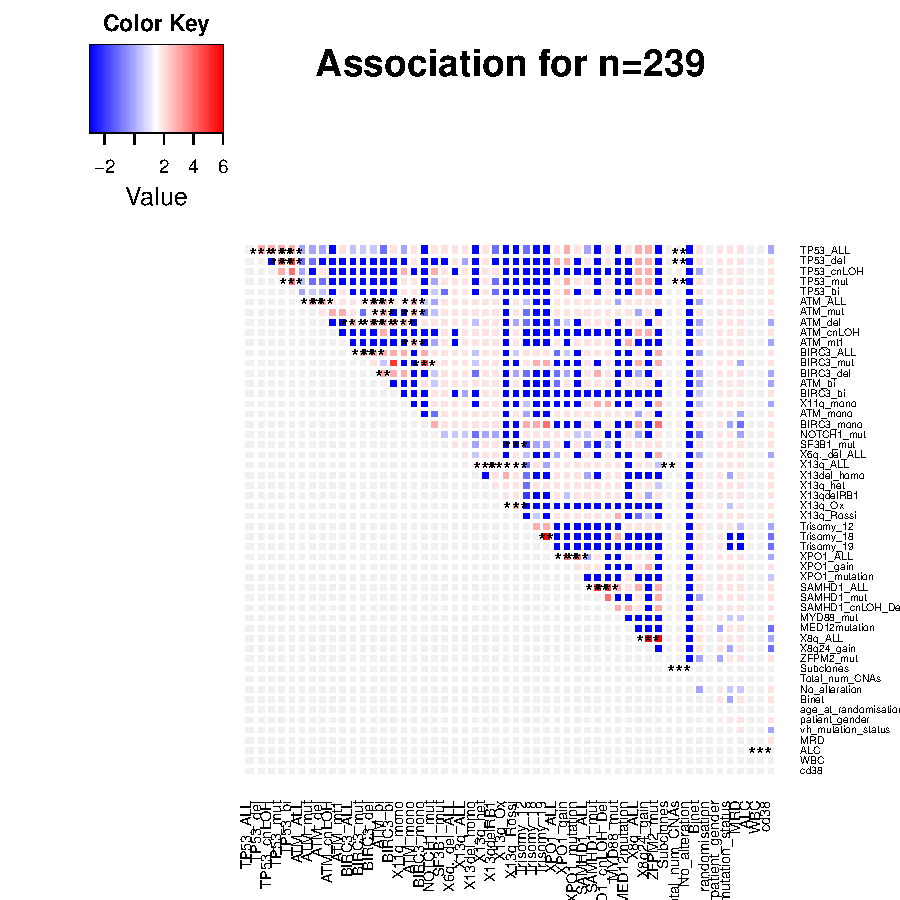
\includegraphics{HICF1_Finalreportv1-008}
\section*{Model building - from here, only 209 data points will be used}
\section*{Association on model data}
This was calculated to see if there are Colinearities that have to be taken into account for the modelling. There are fewer associations than in the 239 data set. 


\begin{landscape}
% Table created by stargazer v.5.1 by Marek Hlavac, Harvard University. E-mail: hlavac at fas.harvard.edu
% Date and time: Tue, Jul 29, 2014 - 16:08:21
\begin{table}[!htbp] \centering 
  \caption{Corrected p-values for association between genetic lesions, n=209} 
  \label{} 
\tiny 
\begin{tabular}{@{\extracolsep{0p}} cccccccccccccccccccccccccccccccccccccccccccccccccccccc} 
\\[-1.8ex]\hline 
\hline \\[-1.8ex] 
 & variables & TP53\_ALL & TP53\_del & TP53\_cnLOH & TP53\_mut & TP53\_bi & ATM\_ALL & ATM\_mut & ATM\_del & ATM\_cnLOH & ATM\_mt1 & BIRC3\_ALL & BIRC3\_mut & BIRC3\_del & ATM\_bi & BIRC3\_bi & X11q\_mono & ATM\_mono & BIRC3\_mono & NOTCH1\_mut & SF3B1\_mut & X6q.\_del\_ALL & X13q\_ALL & X13del\_homo & X13q\_het & X13qdelRB1 & X13q\_Ox & X13q\_Rossi & Trisomy\_12 & Trisomy\_18 & Trisomy\_19 & XPO1\_ALL & XPO1\_gain & XPO1\_mutation & SAMHD1\_ALL & SAMHD1\_mut & SAMHD1\_cnLOH\_Del & MYD88\_mut & MED12mutation & X8q\_ALL & X8q24\_gain & ZFPM2\_mut & Subclones & Total\_num\_CNAs & No\_alteration & Binet & age\_at\_randomisation & patient\_gender & vh\_mutation\_status & MRD & ALC & WBC & cd38 \\ 
\hline \\[-1.8ex] 
1 & TP53\_ALL & $$ & $0.001$ & $1$ & $0$ & $0$ & $1$ & $1$ & $1$ & $1$ & $1$ & $1$ & $1$ & $1$ & $1$ & $1$ & $1$ & $1$ & $1$ & $1$ & $1$ & $1$ & $1$ & $1$ & $1$ & $1$ & $1$ & $0.409$ & $1$ & $1$ & $1$ & $1$ & $1$ & $1$ & $1$ & $1$ & $1$ & $1$ & $1$ & $1$ & $1$ & $1$ & $1$ & $0.010$ & $1$ & $1$ & $1$ & $1$ & $1$ & $1$ & $1$ & $1$ & $1$ \\ 
2 & TP53\_del & $$ & $$ & $1$ & $0$ & $0$ & $1$ & $1$ & $1$ & $1$ & $1$ & $1$ & $1$ & $1$ & $1$ & $1$ & $1$ & $1$ & $1$ & $1$ & $1$ & $1$ & $1$ & $1$ & $1$ & $1$ & $1$ & $1$ & $1$ & $1$ & $1$ & $1$ & $1$ & $1$ & $1$ & $1$ & $1$ & $1$ & $1$ & $1$ & $1$ & $1$ & $1$ & $0.010$ & $1$ & $1$ & $1$ & $1$ & $1$ & $1$ & $1$ & $1$ & $1$ \\ 
3 & TP53\_cnLOH & $$ & $$ & $$ & $1$ & $1$ & $1$ & $1$ & $1$ & $1$ & $1$ & $1$ & $1$ & $1$ & $1$ & $1$ & $1$ & $1$ & $1$ & $1$ & $1$ & $1$ & $1$ & $1$ & $1$ & $1$ & $1$ & $1$ & $1$ & $1$ & $1$ & $1$ & $1$ & $1$ & $1$ & $1$ & $1$ & $1$ & $1$ & $1$ & $1$ & $1$ & $1$ & $1$ & $1$ & $1$ & $1$ & $1$ & $1$ & $1$ & $1$ & $1$ & $1$ \\ 
4 & TP53\_mut & $$ & $$ & $$ & $$ & $0$ & $1$ & $1$ & $1$ & $1$ & $1$ & $1$ & $1$ & $1$ & $1$ & $1$ & $1$ & $1$ & $1$ & $1$ & $1$ & $1$ & $1$ & $1$ & $1$ & $1$ & $1$ & $1$ & $1$ & $1$ & $1$ & $1$ & $1$ & $1$ & $1$ & $1$ & $1$ & $1$ & $1$ & $1$ & $1$ & $1$ & $1$ & $0.003$ & $1$ & $1$ & $1$ & $1$ & $1$ & $1$ & $1$ & $1$ & $1$ \\ 
5 & TP53\_bi & $$ & $$ & $$ & $$ & $$ & $1$ & $1$ & $1$ & $1$ & $1$ & $1$ & $1$ & $1$ & $1$ & $1$ & $1$ & $1$ & $1$ & $1$ & $1$ & $1$ & $1$ & $1$ & $1$ & $1$ & $1$ & $1$ & $1$ & $1$ & $1$ & $1$ & $1$ & $1$ & $1$ & $1$ & $1$ & $1$ & $1$ & $1$ & $1$ & $1$ & $1$ & $0.023$ & $1$ & $1$ & $1$ & $1$ & $1$ & $1$ & $1$ & $1$ & $1$ \\ 
6 & ATM\_ALL & $$ & $$ & $$ & $$ & $$ & $$ & $0$ & $0$ & $1$ & $1$ & $0.014$ & $1$ & $0$ & $0.001$ & $1$ & $0.570$ & $0$ & $1$ & $1$ & $1$ & $1$ & $1$ & $1$ & $1$ & $1$ & $0.011$ & $1$ & $1$ & $1$ & $1$ & $1$ & $1$ & $1$ & $1$ & $1$ & $1$ & $1$ & $1$ & $1$ & $1$ & $1$ & $1$ & $1$ & $1$ & $1$ & $1$ & $1$ & $1$ & $1$ & $1$ & $1$ & $1$ \\ 
7 & ATM\_mut & $$ & $$ & $$ & $$ & $$ & $$ & $$ & $1$ & $1$ & $0.127$ & $1$ & $1$ & $1$ & $0$ & $1$ & $1$ & $0$ & $1$ & $1$ & $1$ & $1$ & $1$ & $1$ & $1$ & $1$ & $0.283$ & $1$ & $1$ & $1$ & $1$ & $1$ & $1$ & $1$ & $1$ & $1$ & $1$ & $1$ & $1$ & $1$ & $1$ & $1$ & $1$ & $1$ & $1$ & $1$ & $1$ & $1$ & $1$ & $1$ & $1$ & $1$ & $1$ \\ 
8 & ATM\_del & $$ & $$ & $$ & $$ & $$ & $$ & $$ & $$ & $1$ & $1$ & $0$ & $1$ & $0$ & $0$ & $1$ & $0$ & $1$ & $1$ & $1$ & $1$ & $1$ & $1$ & $1$ & $1$ & $1$ & $1$ & $1$ & $1$ & $1$ & $1$ & $1$ & $1$ & $1$ & $1$ & $1$ & $1$ & $1$ & $1$ & $1$ & $1$ & $1$ & $1$ & $0.555$ & $1$ & $1$ & $1$ & $1$ & $1$ & $1$ & $1$ & $1$ & $1$ \\ 
9 & ATM\_cnLOH & $$ & $$ & $$ & $$ & $$ & $$ & $$ & $$ & $$ & $1$ & $1$ & $1$ & $1$ & $0.368$ & $1$ & $1$ & $1$ & $1$ & $1$ & $1$ & $1$ & $1$ & $1$ & $1$ & $1$ & $1$ & $1$ & $1$ & $1$ & $1$ & $1$ & $1$ & $1$ & $1$ & $1$ & $1$ & $1$ & $1$ & $1$ & $1$ & $1$ & $1$ & $1$ & $1$ & $1$ & $1$ & $1$ & $1$ & $1$ & $1$ & $1$ & $1$ \\ 
10 & ATM\_mt1 & $$ & $$ & $$ & $$ & $$ & $$ & $$ & $$ & $$ & $$ & $1$ & $1$ & $1$ & $1$ & $1$ & $1$ & $0.001$ & $1$ & $1$ & $1$ & $1$ & $1$ & $1$ & $1$ & $1$ & $1$ & $1$ & $1$ & $1$ & $1$ & $1$ & $1$ & $1$ & $1$ & $1$ & $1$ & $1$ & $1$ & $1$ & $1$ & $1$ & $1$ & $1$ & $1$ & $1$ & $1$ & $1$ & $1$ & $1$ & $1$ & $1$ & $1$ \\ 
11 & BIRC3\_ALL & $$ & $$ & $$ & $$ & $$ & $$ & $$ & $$ & $$ & $$ & $$ & $0$ & $0$ & $0.021$ & $1$ & $0.189$ & $1$ & $0.012$ & $1$ & $1$ & $1$ & $1$ & $1$ & $1$ & $1$ & $1$ & $1$ & $1$ & $1$ & $1$ & $1$ & $1$ & $1$ & $1$ & $1$ & $1$ & $1$ & $1$ & $1$ & $1$ & $1$ & $1$ & $1$ & $1$ & $1$ & $1$ & $1$ & $1$ & $1$ & $1$ & $1$ & $1$ \\ 
12 & BIRC3\_mut & $$ & $$ & $$ & $$ & $$ & $$ & $$ & $$ & $$ & $$ & $$ & $$ & $1$ & $1$ & $0.024$ & $1$ & $1$ & $0$ & $1$ & $1$ & $1$ & $1$ & $1$ & $1$ & $1$ & $1$ & $1$ & $1$ & $1$ & $1$ & $1$ & $1$ & $1$ & $1$ & $1$ & $1$ & $1$ & $1$ & $1$ & $1$ & $1$ & $1$ & $1$ & $1$ & $1$ & $1$ & $1$ & $1$ & $1$ & $1$ & $1$ & $1$ \\ 
13 & BIRC3\_del & $$ & $$ & $$ & $$ & $$ & $$ & $$ & $$ & $$ & $$ & $$ & $$ & $$ & $0.003$ & $0.590$ & $0.018$ & $1$ & $1$ & $1$ & $1$ & $1$ & $1$ & $1$ & $1$ & $1$ & $1$ & $1$ & $1$ & $1$ & $1$ & $1$ & $1$ & $1$ & $1$ & $1$ & $1$ & $1$ & $1$ & $1$ & $1$ & $1$ & $1$ & $1$ & $1$ & $1$ & $1$ & $1$ & $1$ & $1$ & $1$ & $1$ & $1$ \\ 
14 & ATM\_bi & $$ & $$ & $$ & $$ & $$ & $$ & $$ & $$ & $$ & $$ & $$ & $$ & $$ & $$ & $1$ & $1$ & $1$ & $1$ & $1$ & $1$ & $1$ & $1$ & $1$ & $1$ & $1$ & $1$ & $1$ & $1$ & $1$ & $1$ & $1$ & $1$ & $1$ & $1$ & $1$ & $1$ & $1$ & $1$ & $1$ & $1$ & $1$ & $1$ & $0.445$ & $1$ & $1$ & $1$ & $1$ & $1$ & $1$ & $1$ & $1$ & $1$ \\ 
15 & BIRC3\_bi & $$ & $$ & $$ & $$ & $$ & $$ & $$ & $$ & $$ & $$ & $$ & $$ & $$ & $$ & $$ & $1$ & $1$ & $1$ & $1$ & $1$ & $1$ & $1$ & $1$ & $1$ & $1$ & $1$ & $1$ & $1$ & $1$ & $1$ & $1$ & $1$ & $1$ & $1$ & $1$ & $1$ & $1$ & $1$ & $1$ & $1$ & $1$ & $1$ & $1$ & $1$ & $1$ & $1$ & $1$ & $1$ & $1$ & $1$ & $1$ & $1$ \\ 
16 & X11q\_mono & $$ & $$ & $$ & $$ & $$ & $$ & $$ & $$ & $$ & $$ & $$ & $$ & $$ & $$ & $$ & $$ & $1$ & $1$ & $1$ & $1$ & $1$ & $1$ & $1$ & $1$ & $1$ & $1$ & $1$ & $1$ & $1$ & $1$ & $1$ & $1$ & $1$ & $1$ & $1$ & $1$ & $1$ & $1$ & $1$ & $1$ & $1$ & $1$ & $1$ & $1$ & $1$ & $1$ & $1$ & $1$ & $1$ & $1$ & $1$ & $1$ \\ 
17 & ATM\_mono & $$ & $$ & $$ & $$ & $$ & $$ & $$ & $$ & $$ & $$ & $$ & $$ & $$ & $$ & $$ & $$ & $$ & $1$ & $1$ & $1$ & $1$ & $1$ & $1$ & $1$ & $1$ & $1$ & $1$ & $1$ & $1$ & $1$ & $1$ & $1$ & $1$ & $1$ & $1$ & $1$ & $1$ & $1$ & $1$ & $1$ & $1$ & $1$ & $1$ & $1$ & $1$ & $1$ & $1$ & $1$ & $1$ & $1$ & $1$ & $1$ \\ 
18 & BIRC3\_mono & $$ & $$ & $$ & $$ & $$ & $$ & $$ & $$ & $$ & $$ & $$ & $$ & $$ & $$ & $$ & $$ & $$ & $$ & $1$ & $1$ & $1$ & $1$ & $1$ & $1$ & $1$ & $1$ & $1$ & $1$ & $1$ & $1$ & $1$ & $1$ & $1$ & $1$ & $1$ & $1$ & $1$ & $1$ & $1$ & $1$ & $1$ & $1$ & $1$ & $1$ & $1$ & $1$ & $1$ & $1$ & $1$ & $1$ & $1$ & $1$ \\ 
19 & NOTCH1\_mut & $$ & $$ & $$ & $$ & $$ & $$ & $$ & $$ & $$ & $$ & $$ & $$ & $$ & $$ & $$ & $$ & $$ & $$ & $$ & $1$ & $1$ & $1$ & $1$ & $1$ & $1$ & $1$ & $0.125$ & $1$ & $1$ & $1$ & $1$ & $1$ & $1$ & $1$ & $1$ & $1$ & $1$ & $1$ & $1$ & $1$ & $1$ & $1$ & $1$ & $1$ & $1$ & $1$ & $1$ & $1$ & $1$ & $1$ & $1$ & $1$ \\ 
20 & SF3B1\_mut & $$ & $$ & $$ & $$ & $$ & $$ & $$ & $$ & $$ & $$ & $$ & $$ & $$ & $$ & $$ & $$ & $$ & $$ & $$ & $$ & $1$ & $1$ & $1$ & $1$ & $1$ & $0.898$ & $0$ & $1$ & $1$ & $1$ & $1$ & $1$ & $1$ & $1$ & $1$ & $1$ & $1$ & $1$ & $1$ & $1$ & $1$ & $1$ & $1$ & $1$ & $1$ & $1$ & $1$ & $1$ & $1$ & $1$ & $1$ & $1$ \\ 
21 & X6q.\_del\_ALL & $$ & $$ & $$ & $$ & $$ & $$ & $$ & $$ & $$ & $$ & $$ & $$ & $$ & $$ & $$ & $$ & $$ & $$ & $$ & $$ & $$ & $1$ & $1$ & $1$ & $1$ & $1$ & $1$ & $1$ & $1$ & $1$ & $1$ & $1$ & $1$ & $1$ & $1$ & $1$ & $1$ & $1$ & $1$ & $1$ & $1$ & $1$ & $0.121$ & $1$ & $1$ & $1$ & $1$ & $1$ & $1$ & $1$ & $1$ & $1$ \\ 
22 & X13q\_ALL & $$ & $$ & $$ & $$ & $$ & $$ & $$ & $$ & $$ & $$ & $$ & $$ & $$ & $$ & $$ & $$ & $$ & $$ & $$ & $$ & $$ & $$ & $1$ & $0$ & $0.004$ & $0.662$ & $0$ & $0.081$ & $1$ & $1$ & $1$ & $1$ & $1$ & $1$ & $1$ & $1$ & $1$ & $1$ & $1$ & $1$ & $1$ & $0.005$ & $0.721$ & $1$ & $1$ & $1$ & $1$ & $1$ & $1$ & $1$ & $1$ & $1$ \\ 
23 & X13del\_homo & $$ & $$ & $$ & $$ & $$ & $$ & $$ & $$ & $$ & $$ & $$ & $$ & $$ & $$ & $$ & $$ & $$ & $$ & $$ & $$ & $$ & $$ & $$ & $0.027$ & $1$ & $0.716$ & $0.293$ & $1$ & $1$ & $1$ & $1$ & $1$ & $1$ & $1$ & $1$ & $1$ & $1$ & $1$ & $1$ & $1$ & $1$ & $1$ & $1$ & $1$ & $1$ & $1$ & $1$ & $1$ & $1$ & $1$ & $1$ & $1$ \\ 
24 & X13q\_het & $$ & $$ & $$ & $$ & $$ & $$ & $$ & $$ & $$ & $$ & $$ & $$ & $$ & $$ & $$ & $$ & $$ & $$ & $$ & $$ & $$ & $$ & $$ & $$ & $0.014$ & $1$ & $0.118$ & $0.803$ & $1$ & $1$ & $1$ & $1$ & $1$ & $1$ & $1$ & $1$ & $1$ & $1$ & $1$ & $1$ & $1$ & $1$ & $1$ & $1$ & $1$ & $1$ & $1$ & $1$ & $1$ & $1$ & $1$ & $1$ \\ 
25 & X13qdelRB1 & $$ & $$ & $$ & $$ & $$ & $$ & $$ & $$ & $$ & $$ & $$ & $$ & $$ & $$ & $$ & $$ & $$ & $$ & $$ & $$ & $$ & $$ & $$ & $$ & $$ & $1$ & $1$ & $1$ & $1$ & $1$ & $1$ & $1$ & $1$ & $1$ & $1$ & $1$ & $1$ & $1$ & $1$ & $1$ & $1$ & $1$ & $1$ & $1$ & $1$ & $1$ & $1$ & $1$ & $1$ & $1$ & $1$ & $1$ \\ 
26 & X13q\_Ox & $$ & $$ & $$ & $$ & $$ & $$ & $$ & $$ & $$ & $$ & $$ & $$ & $$ & $$ & $$ & $$ & $$ & $$ & $$ & $$ & $$ & $$ & $$ & $$ & $$ & $$ & $0$ & $1$ & $1$ & $1$ & $1$ & $1$ & $1$ & $1$ & $1$ & $1$ & $1$ & $1$ & $1$ & $1$ & $1$ & $1$ & $1$ & $1$ & $1$ & $1$ & $1$ & $1$ & $1$ & $1$ & $1$ & $1$ \\ 
27 & X13q\_Rossi & $$ & $$ & $$ & $$ & $$ & $$ & $$ & $$ & $$ & $$ & $$ & $$ & $$ & $$ & $$ & $$ & $$ & $$ & $$ & $$ & $$ & $$ & $$ & $$ & $$ & $$ & $$ & $0.017$ & $1$ & $1$ & $1$ & $1$ & $1$ & $1$ & $1$ & $1$ & $1$ & $1$ & $1$ & $1$ & $1$ & $0.430$ & $1$ & $1$ & $1$ & $1$ & $1$ & $1$ & $1$ & $1$ & $1$ & $1$ \\ 
28 & Trisomy\_12 & $$ & $$ & $$ & $$ & $$ & $$ & $$ & $$ & $$ & $$ & $$ & $$ & $$ & $$ & $$ & $$ & $$ & $$ & $$ & $$ & $$ & $$ & $$ & $$ & $$ & $$ & $$ & $$ & $1$ & $1$ & $1$ & $1$ & $1$ & $1$ & $1$ & $1$ & $1$ & $1$ & $1$ & $1$ & $1$ & $1$ & $1$ & $1$ & $1$ & $1$ & $1$ & $1$ & $1$ & $1$ & $1$ & $1$ \\ 
29 & Trisomy\_18 & $$ & $$ & $$ & $$ & $$ & $$ & $$ & $$ & $$ & $$ & $$ & $$ & $$ & $$ & $$ & $$ & $$ & $$ & $$ & $$ & $$ & $$ & $$ & $$ & $$ & $$ & $$ & $$ & $$ & $0.002$ & $1$ & $1$ & $1$ & $1$ & $1$ & $1$ & $1$ & $1$ & $1$ & $1$ & $1$ & $1$ & $1$ & $1$ & $1$ & $1$ & $1$ & $1$ & $1$ & $1$ & $1$ & $1$ \\ 
30 & Trisomy\_19 & $$ & $$ & $$ & $$ & $$ & $$ & $$ & $$ & $$ & $$ & $$ & $$ & $$ & $$ & $$ & $$ & $$ & $$ & $$ & $$ & $$ & $$ & $$ & $$ & $$ & $$ & $$ & $$ & $$ & $$ & $1$ & $1$ & $1$ & $1$ & $1$ & $1$ & $1$ & $1$ & $1$ & $1$ & $1$ & $1$ & $1$ & $1$ & $1$ & $1$ & $1$ & $1$ & $1$ & $1$ & $1$ & $1$ \\ 
31 & XPO1\_ALL & $$ & $$ & $$ & $$ & $$ & $$ & $$ & $$ & $$ & $$ & $$ & $$ & $$ & $$ & $$ & $$ & $$ & $$ & $$ & $$ & $$ & $$ & $$ & $$ & $$ & $$ & $$ & $$ & $$ & $$ & $$ & $0$ & $0$ & $1$ & $1$ & $1$ & $1$ & $1$ & $1$ & $1$ & $1$ & $1$ & $1$ & $1$ & $1$ & $1$ & $1$ & $1$ & $1$ & $1$ & $1$ & $1$ \\ 
32 & XPO1\_gain & $$ & $$ & $$ & $$ & $$ & $$ & $$ & $$ & $$ & $$ & $$ & $$ & $$ & $$ & $$ & $$ & $$ & $$ & $$ & $$ & $$ & $$ & $$ & $$ & $$ & $$ & $$ & $$ & $$ & $$ & $$ & $$ & $1$ & $1$ & $1$ & $1$ & $1$ & $1$ & $1$ & $1$ & $1$ & $1$ & $0.945$ & $1$ & $1$ & $1$ & $1$ & $1$ & $1$ & $1$ & $1$ & $1$ \\ 
33 & XPO1\_mutation & $$ & $$ & $$ & $$ & $$ & $$ & $$ & $$ & $$ & $$ & $$ & $$ & $$ & $$ & $$ & $$ & $$ & $$ & $$ & $$ & $$ & $$ & $$ & $$ & $$ & $$ & $$ & $$ & $$ & $$ & $$ & $$ & $$ & $1$ & $1$ & $1$ & $1$ & $1$ & $1$ & $1$ & $1$ & $1$ & $1$ & $1$ & $1$ & $1$ & $1$ & $1$ & $1$ & $1$ & $1$ & $1$ \\ 
34 & SAMHD1\_ALL & $$ & $$ & $$ & $$ & $$ & $$ & $$ & $$ & $$ & $$ & $$ & $$ & $$ & $$ & $$ & $$ & $$ & $$ & $$ & $$ & $$ & $$ & $$ & $$ & $$ & $$ & $$ & $$ & $$ & $$ & $$ & $$ & $$ & $$ & $0$ & $0$ & $1$ & $1$ & $1$ & $1$ & $1$ & $1$ & $1$ & $1$ & $1$ & $1$ & $1$ & $1$ & $1$ & $1$ & $1$ & $1$ \\ 
35 & SAMHD1\_mut & $$ & $$ & $$ & $$ & $$ & $$ & $$ & $$ & $$ & $$ & $$ & $$ & $$ & $$ & $$ & $$ & $$ & $$ & $$ & $$ & $$ & $$ & $$ & $$ & $$ & $$ & $$ & $$ & $$ & $$ & $$ & $$ & $$ & $$ & $$ & $0.496$ & $1$ & $1$ & $1$ & $1$ & $1$ & $1$ & $1$ & $1$ & $1$ & $1$ & $1$ & $1$ & $1$ & $1$ & $1$ & $1$ \\ 
36 & SAMHD1\_cnLOH\_Del & $$ & $$ & $$ & $$ & $$ & $$ & $$ & $$ & $$ & $$ & $$ & $$ & $$ & $$ & $$ & $$ & $$ & $$ & $$ & $$ & $$ & $$ & $$ & $$ & $$ & $$ & $$ & $$ & $$ & $$ & $$ & $$ & $$ & $$ & $$ & $$ & $1$ & $1$ & $1$ & $1$ & $1$ & $1$ & $1$ & $1$ & $1$ & $1$ & $1$ & $1$ & $1$ & $1$ & $1$ & $1$ \\ 
37 & MYD88\_mut & $$ & $$ & $$ & $$ & $$ & $$ & $$ & $$ & $$ & $$ & $$ & $$ & $$ & $$ & $$ & $$ & $$ & $$ & $$ & $$ & $$ & $$ & $$ & $$ & $$ & $$ & $$ & $$ & $$ & $$ & $$ & $$ & $$ & $$ & $$ & $$ & $$ & $1$ & $1$ & $1$ & $1$ & $1$ & $1$ & $1$ & $1$ & $1$ & $1$ & $1$ & $1$ & $1$ & $1$ & $1$ \\ 
38 & MED12mutation & $$ & $$ & $$ & $$ & $$ & $$ & $$ & $$ & $$ & $$ & $$ & $$ & $$ & $$ & $$ & $$ & $$ & $$ & $$ & $$ & $$ & $$ & $$ & $$ & $$ & $$ & $$ & $$ & $$ & $$ & $$ & $$ & $$ & $$ & $$ & $$ & $$ & $$ & $1$ & $1$ & $1$ & $1$ & $1$ & $1$ & $1$ & $1$ & $1$ & $1$ & $1$ & $1$ & $1$ & $1$ \\ 
39 & X8q\_ALL & $$ & $$ & $$ & $$ & $$ & $$ & $$ & $$ & $$ & $$ & $$ & $$ & $$ & $$ & $$ & $$ & $$ & $$ & $$ & $$ & $$ & $$ & $$ & $$ & $$ & $$ & $$ & $$ & $$ & $$ & $$ & $$ & $$ & $$ & $$ & $$ & $$ & $$ & $$ & $0$ & $0.036$ & $1$ & $1$ & $1$ & $1$ & $1$ & $1$ & $1$ & $1$ & $1$ & $1$ & $1$ \\ 
40 & X8q24\_gain & $$ & $$ & $$ & $$ & $$ & $$ & $$ & $$ & $$ & $$ & $$ & $$ & $$ & $$ & $$ & $$ & $$ & $$ & $$ & $$ & $$ & $$ & $$ & $$ & $$ & $$ & $$ & $$ & $$ & $$ & $$ & $$ & $$ & $$ & $$ & $$ & $$ & $$ & $$ & $$ & $1$ & $1$ & $1$ & $1$ & $1$ & $1$ & $1$ & $1$ & $1$ & $1$ & $1$ & $1$ \\ 
41 & ZFPM2\_mut & $$ & $$ & $$ & $$ & $$ & $$ & $$ & $$ & $$ & $$ & $$ & $$ & $$ & $$ & $$ & $$ & $$ & $$ & $$ & $$ & $$ & $$ & $$ & $$ & $$ & $$ & $$ & $$ & $$ & $$ & $$ & $$ & $$ & $$ & $$ & $$ & $$ & $$ & $$ & $$ & $$ & $1$ & $1$ & $1$ & $1$ & $1$ & $1$ & $1$ & $1$ & $1$ & $1$ & $1$ \\ 
42 & Subclones & $$ & $$ & $$ & $$ & $$ & $$ & $$ & $$ & $$ & $$ & $$ & $$ & $$ & $$ & $$ & $$ & $$ & $$ & $$ & $$ & $$ & $$ & $$ & $$ & $$ & $$ & $$ & $$ & $$ & $$ & $$ & $$ & $$ & $$ & $$ & $$ & $$ & $$ & $$ & $$ & $$ & $$ & $0$ & $1$ & $1$ & $1$ & $1$ & $1$ & $1$ & $1$ & $1$ & $1$ \\ 
43 & Total\_num\_CNAs & $$ & $$ & $$ & $$ & $$ & $$ & $$ & $$ & $$ & $$ & $$ & $$ & $$ & $$ & $$ & $$ & $$ & $$ & $$ & $$ & $$ & $$ & $$ & $$ & $$ & $$ & $$ & $$ & $$ & $$ & $$ & $$ & $$ & $$ & $$ & $$ & $$ & $$ & $$ & $$ & $$ & $$ & $$ & $1$ & $1$ & $1$ & $1$ & $1$ & $1$ & $1$ & $1$ & $1$ \\ 
44 & No\_alteration & $$ & $$ & $$ & $$ & $$ & $$ & $$ & $$ & $$ & $$ & $$ & $$ & $$ & $$ & $$ & $$ & $$ & $$ & $$ & $$ & $$ & $$ & $$ & $$ & $$ & $$ & $$ & $$ & $$ & $$ & $$ & $$ & $$ & $$ & $$ & $$ & $$ & $$ & $$ & $$ & $$ & $$ & $$ & $$ & $1$ & $1$ & $1$ & $1$ & $1$ & $1$ & $1$ & $1$ \\ 
45 & Binet & $$ & $$ & $$ & $$ & $$ & $$ & $$ & $$ & $$ & $$ & $$ & $$ & $$ & $$ & $$ & $$ & $$ & $$ & $$ & $$ & $$ & $$ & $$ & $$ & $$ & $$ & $$ & $$ & $$ & $$ & $$ & $$ & $$ & $$ & $$ & $$ & $$ & $$ & $$ & $$ & $$ & $$ & $$ & $$ & $$ & $1$ & $1$ & $1$ & $1$ & $1$ & $1$ & $1$ \\ 
46 & age\_at\_randomisation & $$ & $$ & $$ & $$ & $$ & $$ & $$ & $$ & $$ & $$ & $$ & $$ & $$ & $$ & $$ & $$ & $$ & $$ & $$ & $$ & $$ & $$ & $$ & $$ & $$ & $$ & $$ & $$ & $$ & $$ & $$ & $$ & $$ & $$ & $$ & $$ & $$ & $$ & $$ & $$ & $$ & $$ & $$ & $$ & $$ & $$ & $1$ & $1$ & $1$ & $1$ & $1$ & $1$ \\ 
47 & patient\_gender & $$ & $$ & $$ & $$ & $$ & $$ & $$ & $$ & $$ & $$ & $$ & $$ & $$ & $$ & $$ & $$ & $$ & $$ & $$ & $$ & $$ & $$ & $$ & $$ & $$ & $$ & $$ & $$ & $$ & $$ & $$ & $$ & $$ & $$ & $$ & $$ & $$ & $$ & $$ & $$ & $$ & $$ & $$ & $$ & $$ & $$ & $$ & $1$ & $1$ & $1$ & $1$ & $1$ \\ 
48 & vh\_mutation\_status & $$ & $$ & $$ & $$ & $$ & $$ & $$ & $$ & $$ & $$ & $$ & $$ & $$ & $$ & $$ & $$ & $$ & $$ & $$ & $$ & $$ & $$ & $$ & $$ & $$ & $$ & $$ & $$ & $$ & $$ & $$ & $$ & $$ & $$ & $$ & $$ & $$ & $$ & $$ & $$ & $$ & $$ & $$ & $$ & $$ & $$ & $$ & $$ & $1$ & $1$ & $1$ & $1$ \\ 
49 & MRD & $$ & $$ & $$ & $$ & $$ & $$ & $$ & $$ & $$ & $$ & $$ & $$ & $$ & $$ & $$ & $$ & $$ & $$ & $$ & $$ & $$ & $$ & $$ & $$ & $$ & $$ & $$ & $$ & $$ & $$ & $$ & $$ & $$ & $$ & $$ & $$ & $$ & $$ & $$ & $$ & $$ & $$ & $$ & $$ & $$ & $$ & $$ & $$ & $$ & $1$ & $1$ & $1$ \\ 
50 & ALC & $$ & $$ & $$ & $$ & $$ & $$ & $$ & $$ & $$ & $$ & $$ & $$ & $$ & $$ & $$ & $$ & $$ & $$ & $$ & $$ & $$ & $$ & $$ & $$ & $$ & $$ & $$ & $$ & $$ & $$ & $$ & $$ & $$ & $$ & $$ & $$ & $$ & $$ & $$ & $$ & $$ & $$ & $$ & $$ & $$ & $$ & $$ & $$ & $$ & $$ & $0$ & $1$ \\ 
51 & WBC & $$ & $$ & $$ & $$ & $$ & $$ & $$ & $$ & $$ & $$ & $$ & $$ & $$ & $$ & $$ & $$ & $$ & $$ & $$ & $$ & $$ & $$ & $$ & $$ & $$ & $$ & $$ & $$ & $$ & $$ & $$ & $$ & $$ & $$ & $$ & $$ & $$ & $$ & $$ & $$ & $$ & $$ & $$ & $$ & $$ & $$ & $$ & $$ & $$ & $$ & $$ & $1$ \\ 
52 & cd38 & $$ & $$ & $$ & $$ & $$ & $$ & $$ & $$ & $$ & $$ & $$ & $$ & $$ & $$ & $$ & $$ & $$ & $$ & $$ & $$ & $$ & $$ & $$ & $$ & $$ & $$ & $$ & $$ & $$ & $$ & $$ & $$ & $$ & $$ & $$ & $$ & $$ & $$ & $$ & $$ & $$ & $$ & $$ & $$ & $$ & $$ & $$ & $$ & $$ & $$ & $$ & $$ \\ 
\hline \\[-1.8ex] 
\end{tabular} 
\end{table} \end{landscape}
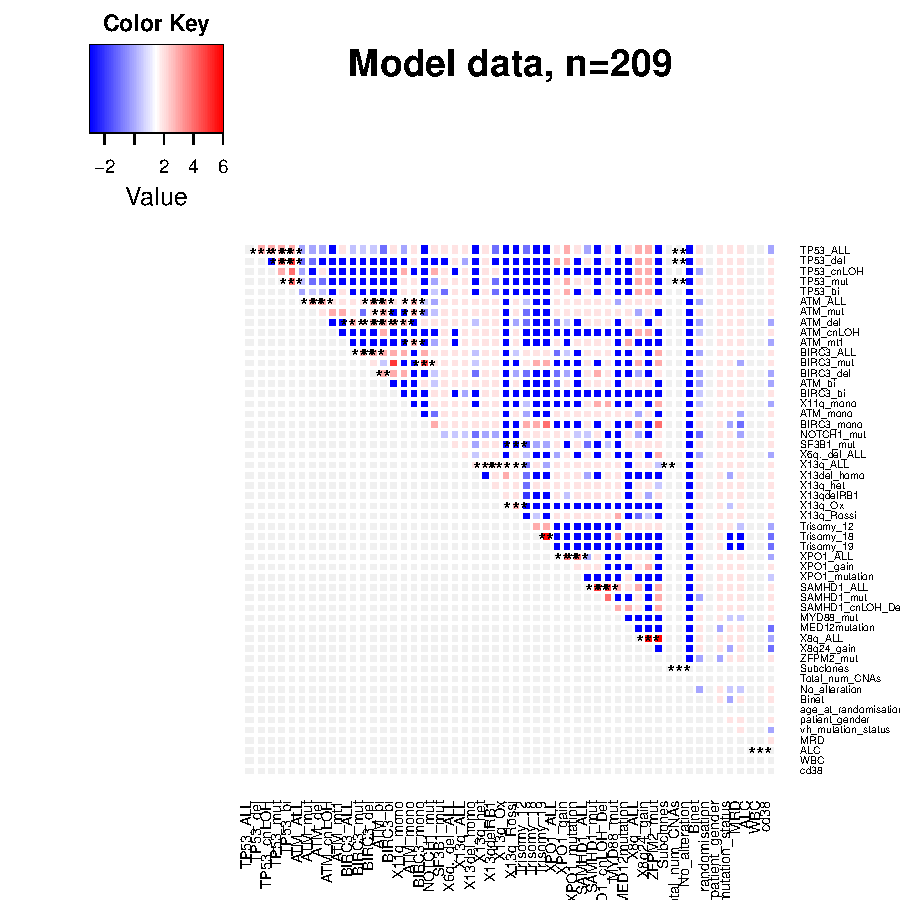
\includegraphics{HICF1_Finalreportv1-013}

\section*{Logistic regression model}
\subsection*{Simple logistic regression models}
For these models, I used the variables that turned out significant in the univariate analysis (model 1-4 in table 5). This is a commonly used procedure, but it can mean that I selected variables that are highly colinear (or co-occuring), TP53 variables for example.
\subsection*{Summarized Model}
For these models, I summarized the data even more:
\begin{itemize}
  \item all trisomies are grouped together
  \item for each lesion, I used the broadest variable
\end{itemize}

%\begin{landscape}
% Table created by stargazer v.5.1 by Marek Hlavac, Harvard University. E-mail: hlavac at fas.harvard.edu
% Date and time: Tue, Jul 29, 2014 - 16:08:25
\begin{table}[!htbp] \centering 
  \caption{Multiple log regression, n=209} 
  \label{} 
\tiny 
\begin{tabular}{@{\extracolsep{5pt}}lcccccc} 
\\[-1.8ex]\hline 
\hline \\[-1.8ex] 
 & \multicolumn{6}{c}{\textit{Dependent variable:}} \\ 
\cline{2-7} 
\\[-1.8ex] & \multicolumn{6}{c}{MRD} \\ 
 & uncorrected
all & uncorrected
genetic & corrected
all & corrected
genetic & summarized
genetic & summarized
vhmut \\ 
\hline \\[-1.8ex] 
 Tri\_ALL1 &  &  &  &  & $-$0.83$^{*}$ (0.47) & $-$1.06$^{**}$ (0.54) \\ 
  TP53\_ALL1 & 1.11 (1.31) & 1.49 (1.19) & 1.49 (1.25) & 1.04 (0.93) & 2.71$^{***}$ (0.77) & 2.88$^{***}$ (1.07) \\ 
  TP53\_del1 & 17.95 (9,579.62) & 18.88 (5,618.88) &  &  &  &  \\ 
  TP53\_cnLOH1 & 18.26 (6,522.64) & 18.92 (5,344.79) &  &  &  &  \\ 
  TP53\_mut1 & 17.39 (2,867.15) & 17.51 (2,649.92) & 16.16 (1,138.99) & 16.93 (1,012.72) &  &  \\ 
  TP53\_bi1 & $-$18.12 (9,659.72) & $-$19.23 (4,622.34) &  &  &  &  \\ 
  ATM\_ALL1 & 17.36 (3,180.05) & 1.43 (1.65) & 0.43 (0.47) & 0.35 (0.43) & 0.98$^{***}$ (0.33) & 0.83$^{**}$ (0.37) \\ 
  ATM\_mut1 & $-$17.34 (3,180.05) & $-$1.38 (1.70) &  &  &  &  \\ 
  ATM\_del1 & $-$17.48 (3,180.05) & 0.09 (1.47) & $-$0.29 (0.95) & 0.52 (0.85) &  &  \\ 
  BIRC3\_ALL1 & $-$0.92 (1.44) & $-$1.50 (1.35) &  &  &  &  \\ 
  BIRC3\_del1 & 1.09 (1.53) & 1.37 (1.38) & 0.57 (0.94) & 0.52 (0.87) &  &  \\ 
  ATM\_bi1 & 19.00 (3,180.05) & 1.81 (1.21) & 1.37$^{*}$ (0.72) & 0.78 (0.64) &  &  \\ 
  X11q\_mono1 & 1.56 (1.62) & 0.15 (1.26) &  &  &  &  \\ 
  BIRC3\_mono1 &  &  &  &  &  &  \\ 
  NOTCH1\_mut1 & $-$0.91 (0.60) & $-$0.85 (0.58) &  &  & $-$0.58 (0.50) & $-$0.71 (0.55) \\ 
  Trisomy\_121 & $-$0.60 (0.57) & $-$0.31 (0.50) & $-$1.04$^{**}$ (0.52) & $-$0.79$^{*}$ (0.45) &  &  \\ 
  Trisomy\_181 & $-$15.94 (2,665.11) & $-$16.06 (2,322.88) &  &  &  &  \\ 
  Trisomy\_191 & $-$15.53 (2,495.26) & $-$15.78 (2,197.33) &  &  &  &  \\ 
  XPO1\_gain1 & 1.14 (1.00) & 1.23 (0.98) &  &  &  &  \\ 
  SAMHD1\_ALL1 & $-$0.26 (1.65) & 0.21 (1.33) &  &  & 1.59$^{*}$ (0.83) & 1.37 (0.85) \\ 
  SAMHD1\_mut1 & 18.72 (2,362.11) & 18.51 (2,202.25) &  &  &  &  \\ 
  Subclones & $-$0.11 (0.29) & $-$0.07 (0.25) &  &  &  &  \\ 
  vh\_mutation\_statusunmutated & 0.72$^{*}$ (0.40) &  & 0.75$^{**}$ (0.35) &  &  & 0.89$^{**}$ (0.36) \\ 
  ALC & 0.004 (0.01) &  &  &  &  &  \\ 
  WBC & $-$0.002 (0.01) &  &  &  &  &  \\ 
  SF3B1\_mut1 &  &  &  &  & $-$0.05 (0.37) &  \\ 
  Constant & $-$0.85$^{**}$ (0.39) & $-$0.44 (0.27) & $-$0.87$^{***}$ (0.28) & $-$0.48$^{**}$ (0.21) & $-$0.44$^{*}$ (0.24) & $-$0.87$^{***}$ (0.29) \\ 
 \hline \\[-1.8ex] 
Observations & 178 & 209 & 181 & 209 & 209 & 181 \\ 
Log Likelihood & $-$88.53 & $-$108.17 & $-$100.29 & $-$120.56 & $-$123.10 & $-$101.52 \\ 
Akaike Inf. Crit. & 225.05 & 258.33 & 218.58 & 257.12 & 260.21 & 217.05 \\ 
\hline 
\hline \\[-1.8ex] 
\textit{Note:}  & \multicolumn{6}{l}{$^{*}$p$<$0.1; $^{**}$p$<$0.05; $^{***}$p$<$0.01} \\ 
\end{tabular} 
\end{table} %\end{landscape}
\subsection*{Discussion of different models}
You can see that the model gets better, the simpler it is. It basically makes no sense at all to put everything we have into a regression model, it is better to use the broadest defined variables (Have to discuss this with Chris though). One good thing with the model that uses only genetic data is that it is as good as the model that includes vh mutation status. It is not really better, but apparently, vh mutation status is a measure that is hard to obtain, and not very reliable. We could argue that genetic testing can almost replace vh mutation status as a predictor for MRD. To harden this argument, I calculated the missclassification error for both models and they are almost identical, yet we have more unclassified when using the vh mutation status.

\subsection*{Missclassification Error}

% Table created by stargazer v.5.1 by Marek Hlavac, Harvard University. E-mail: hlavac at fas.harvard.edu
% Date and time: Tue, Jul 29, 2014 - 16:08:26
\begin{table}[!htbp] \centering 
  \caption{Missclassification for summarized models} 
  \label{} 
\tiny 
\begin{tabular}{@{\extracolsep{1p}} cccccccccc} 
\\[-1.8ex]\hline 
\hline \\[-1.8ex] 
 & model & true\_MRD\_neg & correct\_MRD\_neg & false\_MRD\_neg & true\_MRD\_pos & correct\_MRD\_pos & false\_MRD\_pos & missclasserror & unclassified \\ 
\hline \\[-1.8ex] 
1 & sum\_genetic & $107$ & $84$ & $39$ & $102$ & $63$ & $23$ & $0.297$ & $0$ \\ 
2 & sum\_vhmut & $95$ & $68$ & $30$ & $86$ & $56$ & $27$ & $0.315$ & $29$ \\ 
\hline \\[-1.8ex] 
\end{tabular} 
\end{table} 
% # <<echo=FALSE, results=tex>>=
% # library(xtable)
% # glm <- xtable(fit.sum.gen)
% # print(glm)
% # 
% # @
% # 
% # % \subsection*{Logistic regression with Ridge}
% <<Ridge logistic regression, echo=FALSE, eval=TRUE>>=
% library(glmnet)
% x=data.matrix(genclinMRD[,c(1:48, 54, 55, 56)])
% y=genclinMRD$MRD
% ridge.model <- glmnet(x, y, family="binomial", alpha=0)
% ridge.model
% plot(ridge.model)
% summary(ridge.model)
% coef(ridge.model)
% #Crossvalidate to find optimal lambda:
% set.seed(1712)
% cv.ridge= cv.glmnet(x, y, alpha=0, family="binomial")
% plot(cv.ridge)
% bestlambda=cv.ridge$lambda.min
% bestlambda
% 
% #built model with optimal lambda using the predict function to look at the coefficients
% optimized.ridge.model <- predict(ridge.model, s=bestlambda, type="coefficient")
% optimized.ridge.model <- as.data.frame(as.matrix(optimized.ridge.model))
% colnames(optimized.ridge.model)[1]<- "coefficient_ridge"
% optimized.ridge.model$variables <- row.names(optimized.ridge.model)
% row.names(optimized.ridge.model) <- NULL
% 
% 
% @
% 
% \subsection*{Logistic regression with Lasso}
% <<Lasso logistic regression, echo=FALSE, eval=TRUE>>=
% library(glmnet)
% x=data.matrix(genclinMRD[,c(1:48, 54, 55, 56)])
% genclinMRD[51]
% y=as.numeric(genclinMRD$MRD)
% lasso.model <- glmnet(x, y, family="binomial", alpha=1)
% lasso.model
% plot(lasso.model)
% summary(lasso.model)
% coef(lasso.model)
% #Crossvalidate to find optimal lambda:
% set.seed(1712)
% cv.lasso= cv.glmnet(x, y, alpha=1, family="binomial")
% plot(cv.lasso)
% bestlambda=cv.lasso$lambda.min
% bestlambda
% 
% optimized.lasso.model <- predict(lasso.model, s=bestlambda, type="coefficient")
% optimized.lasso.model <- as.data.frame(as.matrix(optimized.lasso.model))
% colnames(optimized.lasso.model)[1]<- "coefficient_lasso"
% optimized.lasso.model$variables <- row.names(optimized.lasso.model)
% row.names(optimized.lasso.model) <- NULL
% @
% 
% \subsection*{Compare Lasso and Ridge Regression Coefficients}
% <<fig=TRUE, eval=TRUE, echo=FALSE>>=
% coefficients <- cbind(optimized.lasso.model, optimized.ridge.model)
% coefficients <- coefficients[2:52, ]
% library(ggplot2)
% ggplot()+geom_point(data=coefficients, aes(x=coefficient_lasso, y=coefficient_ridge))+
% geom_text(data=coefficients, aes(x=coefficient_lasso, y=coefficient_ridge, label = variables), vjust = 0.7, hjust = 1, size=3, col="darkblue")+
%   xlim(-1, 2)+
%   geom_hline(yintercept=0, alpha=0.5)+
%   geom_hline(yintercept=c(-0.1, 0.1), col="darkred", alpha=0.5, linetype="dashed")+
%   geom_vline(xintercept=0, alpha=0.5)
% @
% \subsection*{Find the best model with only important parameters (includes cutoff for ridge regression)}
% <<Model with results from lasso and ridge, echo=FALSE, eval=TRUE>>=
% variables_ridge_lasso_selected <- subset(coefficients, coefficient_lasso !=0)#& abs(coefficients$coefficient_ridge) > 0.4) 
% genclin_ridge_lasso_selected <- genclinMRD[,colnames(genclinMRD)%in%variables_ridge_lasso_selected$variables] 
% genclin_ridge_lasso_selected$MRD <- genclinMRD$MRD
% 
% system.time(best.subset.from.lasso <- bestglm(genclin_ridge_lasso_selected, family=binomial))
% best.subset.from.lasso
% fit_ridge_lasso_selected <- glm(MRD ~ ., family=binomial(logit), data=genclin_ridge_lasso_selected)
% summary(fit_ridge_lasso_selected)
% @
% 
% \subsection*{Elastic net and group selection (Hasties)}
% Grouped selection: automatically include whole groups into the model if one variable amongst them is selected.(Do we want this?)
% 
% 
% 
% \subsection*{Best subset selection}
% Variables that are important from Univariate Analysis (including trends)
% TP53_All
% TP53_morethan5VAF
% ATM_ALL
% ATM_del
% BIRC3_del
% ATM_biallelic
% vh_mutation_status
% 
% <<Best subset selection, echo=FALSE, eval=TRUE>>=
% 
% library(bestglm)
% #UNCORRECTED
% #take significant/trend variables from univariate analysis
% variables_uncorrected_univariate <- subset(genclinv6.pvalues, p.value < 0.1)
% 
% genclin_univariates_selected <-genclinMRD[,colnames(genclinMRD)%in% row.names(variables_uncorrected_univariate)]
% #take out clinical parameters
% genclin_univariates_selected$WBC <- NULL
% genclin_univariates_selected$ALC <- NULL
% genclin_univariates_selected$vh_mutation_status <- NULL
% 
% x=genclin_univariates_selected
% #x <- na.omit(x)
% y=genclinMRD$MRD
% Xy <- cbind(x, y)
% row.names(Xy) <- NULL
% 
% best.subset.selection <- bestglm(Xy, family=binomial)
% best.subset.selection
% 
% #CORRECTED
% #take significant/trend variables from univariate analysis
% variables_corrected_univariate <- subset(genclinv6.pvalues, corrected.p.value < 0.1)
% 
% genclin_univariates_corrected <-genclinMRD[,colnames(genclinMRD)%in% row.names(variables_corrected_univariate)]
% #take out clinical parameters
% genclin_univariates_corrected$vh_mutation_status <- NULL
% 
% x=genclin_univariates_corrected
% #x <- na.omit(x)
% y=genclinMRD$MRD
% Xy <- cbind(x, y)
% row.names(Xy) <- NULL
% 
% best.subset.corrected <- bestglm(Xy, family=binomial)
% best.subset.corrected
% @

\end{document}

